% Options for packages loaded elsewhere
\PassOptionsToPackage{unicode}{hyperref}
\PassOptionsToPackage{hyphens}{url}
%
\documentclass[
]{article}
\usepackage{amsmath,amssymb}
\usepackage{iftex}
\ifPDFTeX
  \usepackage[T1]{fontenc}
  \usepackage[utf8]{inputenc}
  \usepackage{textcomp} % provide euro and other symbols
\else % if luatex or xetex
  \usepackage{unicode-math} % this also loads fontspec
  \defaultfontfeatures{Scale=MatchLowercase}
  \defaultfontfeatures[\rmfamily]{Ligatures=TeX,Scale=1}
\fi
\usepackage{lmodern}
\ifPDFTeX\else
  % xetex/luatex font selection
\fi
% Use upquote if available, for straight quotes in verbatim environments
\IfFileExists{upquote.sty}{\usepackage{upquote}}{}
\IfFileExists{microtype.sty}{% use microtype if available
  \usepackage[]{microtype}
  \UseMicrotypeSet[protrusion]{basicmath} % disable protrusion for tt fonts
}{}
\makeatletter
\@ifundefined{KOMAClassName}{% if non-KOMA class
  \IfFileExists{parskip.sty}{%
    \usepackage{parskip}
  }{% else
    \setlength{\parindent}{0pt}
    \setlength{\parskip}{6pt plus 2pt minus 1pt}}
}{% if KOMA class
  \KOMAoptions{parskip=half}}
\makeatother
\usepackage{xcolor}
\usepackage{longtable,booktabs,array}
\usepackage{calc} % for calculating minipage widths
% Correct order of tables after \paragraph or \subparagraph
\usepackage{etoolbox}
\makeatletter
\patchcmd\longtable{\par}{\if@noskipsec\mbox{}\fi\par}{}{}
\makeatother
% Allow footnotes in longtable head/foot
\IfFileExists{footnotehyper.sty}{\usepackage{footnotehyper}}{\usepackage{footnote}}
\makesavenoteenv{longtable}
\usepackage{graphicx}
\makeatletter
\def\maxwidth{\ifdim\Gin@nat@width>\linewidth\linewidth\else\Gin@nat@width\fi}
\def\maxheight{\ifdim\Gin@nat@height>\textheight\textheight\else\Gin@nat@height\fi}
\makeatother
% Scale images if necessary, so that they will not overflow the page
% margins by default, and it is still possible to overwrite the defaults
% using explicit options in \includegraphics[width, height, ...]{}
\setkeys{Gin}{width=\maxwidth,height=\maxheight,keepaspectratio}
% Set default figure placement to htbp
\makeatletter
\def\fps@figure{htbp}
\makeatother
\setlength{\emergencystretch}{3em} % prevent overfull lines
\providecommand{\tightlist}{%
  \setlength{\itemsep}{0pt}\setlength{\parskip}{0pt}}
\setcounter{secnumdepth}{5}
% definitions for citeproc citations
\NewDocumentCommand\citeproctext{}{}
\NewDocumentCommand\citeproc{mm}{%
  \begingroup\def\citeproctext{#2}\cite{#1}\endgroup}
\makeatletter
 % allow citations to break across lines
 \let\@cite@ofmt\@firstofone
 % avoid brackets around text for \cite:
 \def\@biblabel#1{}
 \def\@cite#1#2{{#1\if@tempswa , #2\fi}}
\makeatother
\newlength{\cslhangindent}
\setlength{\cslhangindent}{1.5em}
\newlength{\csllabelwidth}
\setlength{\csllabelwidth}{3em}
\newenvironment{CSLReferences}[2] % #1 hanging-indent, #2 entry-spacing
 {\begin{list}{}{%
  \setlength{\itemindent}{0pt}
  \setlength{\leftmargin}{0pt}
  \setlength{\parsep}{0pt}
  % turn on hanging indent if param 1 is 1
  \ifodd #1
   \setlength{\leftmargin}{\cslhangindent}
   \setlength{\itemindent}{-1\cslhangindent}
  \fi
  % set entry spacing
  \setlength{\itemsep}{#2\baselineskip}}}
 {\end{list}}
\usepackage{calc}
\newcommand{\CSLBlock}[1]{\hfill\break#1\hfill\break}
\newcommand{\CSLLeftMargin}[1]{\parbox[t]{\csllabelwidth}{\strut#1\strut}}
\newcommand{\CSLRightInline}[1]{\parbox[t]{\linewidth - \csllabelwidth}{\strut#1\strut}}
\newcommand{\CSLIndent}[1]{\hspace{\cslhangindent}#1}
\usepackage{pdflscape}
\newcommand{\blandscape}{\begin{landscape}}
\newcommand{\elandscape}{\end{landscape}}
\usepackage{lineno}
\linenumbers
\usepackage{setspace}
\doublespacing
\usepackage{booktabs}
\usepackage{longtable}
\usepackage{array}
\usepackage{multirow}
\usepackage{wrapfig}
\usepackage{float}
\usepackage{colortbl}
\usepackage{pdflscape}
\usepackage{tabu}
\usepackage{threeparttable}
\usepackage{threeparttablex}
\usepackage[normalem]{ulem}
\usepackage{makecell}
\usepackage{xcolor}
\ifLuaTeX
  \usepackage{selnolig}  % disable illegal ligatures
\fi
\IfFileExists{bookmark.sty}{\usepackage{bookmark}}{\usepackage{hyperref}}
\IfFileExists{xurl.sty}{\usepackage{xurl}}{} % add URL line breaks if available
\urlstyle{same}
\hypersetup{
  pdftitle={Agricultural ecosystems help contain alien conifer spread from forest plantations in Norway},
  pdfauthor={Julien Vollering1,2*; Siri Lie Olsen3,4; Olav Skarpaas2; Leif Appelgren5; Magni Olsen Kyrkjeeide6; Anders Often3; Jakob Sandven7; Odd Stabbetorp3; Øyvind Sørhuus7},
  hidelinks,
  pdfcreator={LaTeX via pandoc}}

\title{Agricultural ecosystems help contain alien conifer spread from forest plantations in Norway}
\author{Julien Vollering\textsuperscript{1,2}* \and Siri Lie Olsen\textsuperscript{3,4} \and Olav Skarpaas\textsuperscript{2} \and Leif Appelgren\textsuperscript{5} \and Magni Olsen Kyrkjeeide\textsuperscript{6} \and Anders Often\textsuperscript{3} \and Jakob Sandven\textsuperscript{7} \and Odd Stabbetorp\textsuperscript{3} \and Øyvind Sørhuus\textsuperscript{7}}
\date{}

\begin{document}
\maketitle

\textsuperscript{1} Department of Environmental Sciences, Western Norway University of Applied
Sciences, Sogndal, Norway

\textsuperscript{2} Department of Research and Collections, Natural History Museum, University
of Oslo, Oslo, Norway

\textsuperscript{3} Norwegian Institute for Nature Research, Oslo, Norway

\textsuperscript{4} Institute of Urbanism and Landscape, The Oslo School of Architecture and
Design, Oslo, Norway

\textsuperscript{5} Ecofact AS, Sandnes, Norway

\textsuperscript{6} Norwegian Institute for Nature Research, Trondheim, Norway

\textsuperscript{7} NORSKOG, Oslo, Norway

*Corresponding author:
\href{mailto:julienvollering@gmail.com}{\nolinkurl{julienvollering@gmail.com}}

\section{Abstract}\label{abstract}

\begin{enumerate}
\def\labelenumi{\arabic{enumi}.}
\item
  Plantations of alien conifer species are common in many countries and may
  become more prevalent in coming decades, as a way to sequester carbon. To
  minimize spillover from plantations into native ecosystems, land managers
  need to know which ecosystems are most susceptible to establishment and
  growth of self-sown individuals (``wildlings'') of a given species. The
  spatial distribution of the first generation of wildlings close to a
  plantation is an early and therefore valuable indicator of ecosystem
  susceptibility to wildlings, but it is also shaped by the pattern of seed
  rain from the plantations, among other factors.
\item
  We used detailed surveys around 76 plantation stands in Norway to estimate
  ecosystem susceptibility to three groups of commonly planted conifer
  species: \emph{Picea sitchensis} / \emph{Picea} \(\times\)\emph{lutzii}, \emph{Picea abies}, and
  \emph{Larix} spp. We created spatially explicit models of wildling abundance as a
  function of ecosystem type, exposure to seed rain, climate, and plantation
  stand characteristics.
\item
  Our surveys registered 27 wildlings per hectare for \emph{P. sitchensis} / \emph{P.}
  \(\times\)\emph{lutzii} (\(\frac{22356}{860}\) ha\textsuperscript{-1}), 6 ha\textsuperscript{-1} for \emph{P. abies}
  (\(\frac{2245}{396}\) ha\textsuperscript{-1}), and 13 ha\textsuperscript{-1} for \emph{Larix}
  spp.(\(\frac{4213}{319}\) ha\textsuperscript{-1}). For all three species groups, we found that
  ecosystem type was responsible for up to three orders of magnitude of
  difference in wildling abundance. When we stratified wildling abundance by
  height class (\(\geq\)~30~cm and \(\geq\)~100~cm), we also found evidence that
  some ecosystems are more conducive to establishment (reaching 30~cm) than
  growth (reaching 100~cm), and vice versa.
\item
  Agricultural ecosystems of various kinds were among the ecosystems least
  susceptible to wildlings of all three groups of conifer species.
\item
  \emph{Synthesis and applications} We encourage managers to exploit the large
  differences in susceptibility between ecosystems to reduce the spread of
  alien conifers. New plantations should be sited among ecosystems with low
  susceptibility only, and efforts to control wildlings should play close
  attention to susceptible ecosystems --- even where these are not exposed to
  much seed rain. In Norway, situating plantations within a landscape matrix
  of agricultural ecosystems is an effective way to reduce alien conifer
  spread.
\end{enumerate}

\section{Keywords}\label{keywords}

alien species, conifer, ecosystem type, establishment, exposure, forestry,
invasibility, plantation, seed dispersal, susceptibility, vulnerability, Wald
Analytical Long-distance Dispersal (WALD)

\newpage

\section{Introduction}\label{introduction}

While there is a long history of using alien conifers in forestry, the practice
of planting conifers at scale in places where they are not native is hardly a
thing of the past. Commercial forestry relies on alien conifer species in many
parts of the world, with 44~\% of plantation forests globally composed mainly of
introduced species (\citeproc{ref-faoGlobalForestResources2020}{FAO, 2020}). Alien conifer species may
also be included in some of the vast afforestation programs against climate
change Te Uru Rākau New Zealand Forest Service (\citeproc{ref-teururakaunewzealandforestserviceOneBillionTrees2018}{2018}). Therefore, it is likely
that alien conifers will continue to be planted across large areas in coming
decades, sometimes in regions where a given species has not previously occurred.

Responsible forestry practice requires that alien species be kept within
plantation boundaries (\citeproc{ref-brunduGlobalGuidelinesSustainable2020}{Brundu et al., 2020}), but alien
conifer plantations generally produce self-sown individuals beyond the
plantation (``wildlings''). It is prudent to prevent wildlings both to protect the
integrity of surrounding ecosystems and to block secondary, potentially invasive
spread (\citeproc{ref-nunezEcologyManagementInvasive2017}{Nuñez et al., 2017}). Costly conifer invasions --- like
pines in South Africa, to name one example --- usually stem from forestry
plantations (\citeproc{ref-esslSelectionCommercialForestry2010}{Essl et al., 2010}; \citeproc{ref-mcconnachieEstimatingEffectPlantations2015}{McConnachie et al., 2015}). Combined with the expectation of
future planting, the potential for invasions underlines the importance of
preventing wildlings from plantations.

Wildlings come about via a process that starts with seed production in the
plantation, then seed dispersal, followed by seedling establishment and growth.
If we focus on seedling establishment and growth, the rate at which wildlings
accumulate in a given location depends on biotic and abiotic conditions there.
Factors like seed bed characteristics, soil moisture, and light availability are
likely among the most important determinants of establishment and early growth
success --- as they are for natural regeneration of conifers
(\citeproc{ref-burnsSilvicsNorthAmerica1990}{Burns \& Honkala, 1990}). Silviculturalists have long used natural
vegetation composition to forecast the regeneration success of particular
conifer species in particular locations
(\citeproc{ref-savillPlantationSilvicultureEurope1997}{Savill et al., 1997}), which supports the expectations that:
1) vegetation integrates influences on wildling establishment and growth, and 2)
different conifer species have different optima for establishment and growth. In
short, wildlings establish and grow more readily in some kinds of ecosystems
than others, depending on the autecology of the species.

The rate at which wildlings accumulate in a location is also controlled by the
amount of seed rain arriving there, via seed production and dispersal.
Regardless of how well a particular location supports establishment and growth
of a particular species, no more wildlings can appear than seeds arrive.
Conversely, low establishment and growth in a location close to a plantations
may be masked by copious seed rain (\citeproc{ref-rougetInferringProcessPattern2003}{Rouget \& Richardson, 2003}). Thus,
we distinguish between a location's \emph{susceptibility} (intrinsic favorability for
establishment and growth) and its \emph{vulnerability} {[}susceptibility multiplied by
exposure to seed rain and other extrinsic factors;
Chae et al. (\citeproc{ref-chaeVulnerabilityResilienceUse2021}{2021}){]}. The same distinction exists between
\emph{invasibility} and \emph{level of invasion}, but these terms refer to invader
richness rather than invader abundance (\citeproc{ref-richardsonPlantInvasionsMerging2006}{Richardson \& Pyšek, 2006}).
By our definitions, vulnerability is the level of risk realized at a specific
location, while susceptibility is the level of risk that may be attributed to
the conditions at that location. Susceptibility is what we can characterize for
an ecosystem type and expect to remain constant across spatial contexts. For
example, at locations where the nearest seed source is unknown, we may assess
the relative risk of wildlings based on ecosystem susceptibility.

In Norway, wildling abundance around alien conifer plantations varies
considerably --- by species, but also among conspecific plantations
(\citeproc{ref-nygaardNaturligSpredningAv1999}{P. H. Nygaard et al., 1999}; \citeproc{ref-nygaardSpreadIntroducedSitka2017}{P. Nygaard \& Øyen, 2017}). Most of
the alien conifer plantations in Norway today were planted between 1950 and
1990, when subsidies encouraged private reforestation/afforestation, especially
along western coastlines, where forests were scarce. In total, about 80~000~ha
were planted with alien conifer species, of which 50~000~ha was Sitka spruce
\emph{Picea sitchensis} or its hybrid, Lutz spruce \emph{Picea} \(\times\)\emph{lutzii}, and
6~500~ha was larch species \emph{Larix} spp.
(\citeproc{ref-miljodirektoratetUtredningAvForbud2019}{Miljødirektoratet \& Landbruksdirektoratet, 2019}). An additional 210~000~ha were planted
with Norway spruce \emph{Picea abies}, which is native but was planted mainly outside
its historical range (\citeproc{ref-miljodirektoratetUtredningAvForbud2019}{Miljødirektoratet \& Landbruksdirektoratet, 2019}). Today,
silvicultural policy in Norway is more restrictive of alien conifers than in
other European countries (\citeproc{ref-potzelsbergerGrowingNonnativeTrees2020}{Pötzelsberger et al., 2020}). Regulations
from 2012 require forest owners to gain approval for new plantations and
implement measures against resulting wildlings. (\citeproc{ref-ForskriftOmUtsetting2012}{Forskrift om utsetting av utenlandske treslag, 2012}).
These policies aim to prevent wildlings from further deteriorating red-listed
ecosystem types --- coastal heathlands especially, but also Atlantic bogs,
semi-natural grasslands, and others (\citeproc{ref-artsdatabankenFremmedartslista20182018}{Artsdatabanken, 2018}; \citeproc{ref-miljodirektoratetUtredningAvForbud2019}{Miljødirektoratet \& Landbruksdirektoratet, 2019}).

Determining ecosystem susceptibility, so that interventions can be prioritized
objectively and with maximum effect, is among the most urgent objectives for
invasion science (\citeproc{ref-pysekScientistsWarningInvasive2020}{Pyšek et al., 2020}). To mitigate the negative
impacts of alien conifer plantations, we need to know which ecosystems are most
susceptible to wildlings (\citeproc{ref-bindewaldSiteSpecificRisk2021}{Bindewald et al., 2021}; \citeproc{ref-potzelsbergerGrowingNonnativeTrees2020}{Pötzelsberger et al., 2020}). In the Norwegian context specifically,
public authorities need a basis for judging where to allow new alien conifer
plantations, and land managers need a basis for efficient monitoring and
control. However, ecosystem susceptibility to alien conifers is not easily
generalized (\citeproc{ref-higginsPineInvasionsSouthern1998}{Higgins \& Richardson, 1998}) --- not across ecosystems nor
across species. Therefore, we must quantify ecosystem susceptibility in a
granular way, by asking: \emph{how likely is establishment and growth of a particular
species, in a particular ecosystem type}? These values of ecosystem
susceptibility provide a basis for long-term management of alien conifers,
because they can be expected to remain constant as seed sources change and
species spread.

Another key knowledge gap is how much ecosystem vulnerability deviates from
ecosystem susceptibility, as a result of differential exposure to seed rain. We
know that that interventions against alien conifer invasions need to focus on
early stages of invasion (\citeproc{ref-nunezEcologyManagementInvasive2017}{Nuñez et al., 2017}), but these early
stages probably produce highly uneven exposure to seed rain, concentrated in
ecosystems that border plantations. Therefore, we want to know whether or not
initial vulnerability --- i.e., first-generation wildling abundance per
ecosystem --- provides a good approximation of ecosystem susceptibility. A good
approximation would suggest that it is generally safe to estimate long-term
ecosystem susceptibility directly from surveys of plantation surroundings.
Conversely, a poor approximation would highlight the importance of
differentiating between vulnerability and susceptibility --- in Norway and
elsewhere --- to avoid highly susceptible ecosystems being overlooked.

This paper addresses the two knowledge gaps described above (ecosystem
susceptibility, correspondence between susceptibility and vulnerability), for
three groups of common alien conifers in Norway. Four aspects of our methodology
deserve highlighting. First, we fully map the wildlings and ecosystem types
around a given plantation, rather than sampling these. The detailed mapping
allows a fine-scaled, spatially-explicit assessment of the relationship between
wildlings and ecosystems. Second, our delineation of ecosystems follows a
typology that is nationally-adopted for land management in Norway. Our estimates
of susceptibility are therefore directly applicable without additional
uncertainty from imperfect correspondence between ecosystem types. Third, we
estimate exposure by reconstructing the spatial distribution of seed rain from
plantations, testing both mechanistic and phenomenological models of seed
dispersal. Seeds from plantation conifers are generally dispersed by wind alone,
and wind-vectored seed dispersal can be estimated with relative confidence
(\citeproc{ref-nathanDispersalKernels2012}{Nathan et al., 2012}). Fourth, we specify our statistical model of the
wildling--ecosystem relationship based on domain knowledge, with explicitly
stated causal assumptions. This approach prioritizes understanding of ecological
processes and promotes constructive discourse around alternative model
specifications (\citeproc{ref-arifApplyingStructuralCausal2023}{Arif \& MacNeil, 2023}).

In summary, we examine plantations of alien conifers in Norway to investigate
the following questions:

\begin{itemize}
\tightlist
\item
  Which ecosystems are most and least susceptible to wildlings of various
  alien conifer species, and by how much do they differ in their
  susceptibility?
\item
  Are differences in susceptibility among ecosystems masked in the realized
  distribution of wildlings, by differences in exposure to seed rain?
\end{itemize}

\section{Materials and methods}\label{materials-and-methods}

\subsection{Field data}\label{field-data}

We registered wildlings and ecosystems around 76 reproductive plantation stands
across Norway, comprising three groups of alien conifers (hereafter: ``species'';
fig.~\ref{fig:sites-map}). The sample contained (1) forty-two sites with Sitka
spruce (\emph{Picea sitchensis}) or its fertile hybrid, Lutz spruce (\emph{P.}
\(\times\)\emph{lutzii}), (2) nineteen with Norway spruce (\emph{Picea abies}), and (3)
fifteen with larch species (\emph{Larix} spp.). Note that Norway spruce is native to
Norway, but the plantations included in this study were located in parts of the
country where its natural distribution is highly restricted. We selected stands
using aerial imagery, aiming for those isolated from conspecific stands. We
collected field data for each stand in one of six field campaigns during the
period 2016-2019 (\citeproc{ref-appelgrenKartleggingAvKortdistansespredning2018}{Appelgren, 2018}; \citeproc{ref-appelgrenKartleggingAvKortdistansespredning2017}{Appelgren \& Torvik, 2017}; \citeproc{ref-kyrkjeeideKartleggingAvKortdistansespredning2017}{Kyrkjeeide et al., 2017}; reported in \citeproc{ref-olsenKartleggingAvKortdistansespredning2016}{Olsen et al., 2016}, \citeproc{ref-olsenKartleggingAvKortdistansespredning2019}{2019}; \citeproc{ref-sandvenKartleggingAvKortdistansespredning2019}{Sandven et al., 2019}).

\begin{figure}
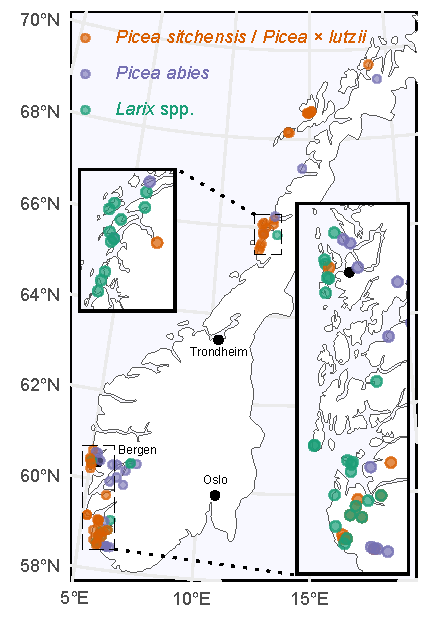
\includegraphics[width=1\linewidth]{figures/sites-map} \caption{Locations of the 76 plantation stands in the sample.}\label{fig:sites-map}
\end{figure}

Within a 2x2 km plot centered on the stand of interest, we mapped all
conspecific stands (except in the 2016 field campaign). Within the central
500x500~m of that plot, we mapped wildlings and ecosystems. We used GPS to
register the point-positions of all wildlings over 30 cm in height, recording a
single position for groups of wildlings occurring with less than 5~m between
them. A few exceptionally dense groups of wildlings were mapped by registering
polygons instead of points and estimating the number of individuals by transect
counts.

Concurrently, we registered polygons for all terrestrial and wetland ecosystems,
following the Nature in Norway classification system (version 2.0 or 2.1, \citeproc{ref-halvorsenNaturNorgeNiN2015}{Halvorsen et al., 2015}; based on the principles summarized in Halvorsen et
al., \citeproc{ref-halvorsenSystematicsEcodiversityEcoSyst2020}{Halvorsen et al., 2020}). This system is the national
standard for land cover mapping and provides full spatial coverage (i.e.~any
location is assignable to an ecosystem). We mapped ecosystems at a scale of
1:5000, which means that any polygon over 250~m\textsuperscript{2} was registered
(\citeproc{ref-brynVeilederKartleggingAv2015}{Bryn \& Halvorsen, 2015}). Regularly patterned occurrence of more than
one ecosystem in polygons smaller than the minimum size were registered as
so-called mosaic polygons.

We estimated or measured (by clinometer) the heights of the 76 central stands.
We also estimated their ages at the time of the field campaign, either by
contacting land owners and municipal officials, or by counting growth rings.
Details of all 76 stands are provided in the Appendix
(table~\ref{tab:sites-table}).

\subsection{Seed rain estimates}\label{seed-rain-estimates}

To account for the influence of seed dispersal on wildling abundance, we needed
estimates of the spatial distribution of seed rain within the 500x500~m plots.
We considered all conspecific stands within a 1 km radius of the plot center to
be potential seed sources, and used two models of seed dispersal to derive
different estimates of relative seed rain in space. Acknowledging the
uncertainty involved in estimating seed dispersal, we explored one
empirically-parameterized, isotropic model and one mechanistically-derived,
anisotropic model.

The first model was a static seed dispersal kernel with parameter estimates
generalized from multiple data sets. Specifically, we selected from Bullock et
al. (\citeproc{ref-bullockSynthesisEmpiricalPlant2017}{2017}) the kernel that performed best for
wind-adapted seeds from 5-15~m tall trees (an Exponential Power function).
Sixty-six of the 76 stands in our data set matched this height range better than
a taller range with a different empirical kernel.

The second model was an anisotropic implementation of the Wald Analytical
Long-distance Dispersal model (WALD, \citeproc{ref-katulMechanisticAnalyticalModels2005}{Katul et al., 2005}),
following Skarpaas \& Shea (\citeproc{ref-skarpaasDispersalPatternsDispersal2007}{2007}). We
parameterized the model with: site- and season-specific wind vectors retrieved
from meteorological data sets {[}MET Norway;
Reistad et al. (\citeproc{ref-reistadHighresolutionHindcastWind2011}{2011}); Haakenstad \& Haugen (\citeproc{ref-haakenstad15yearHighResolution2017}{2017}){]},
wind turbulence estimated from local ecosystem composition, seed release height
based on stand height, and species-specific seed terminal velocities from
literature.

We transformed field-mapped polygons of potential seed sources into hexagonally
gridded point sources, with a density of 0.1~m\textsuperscript{-2} for the first model and
0.01~m\textsuperscript{-2} for the second model (to reduce computation time). Then we applied
our two dispersal models to estimate the distribution of relative seed rain from
all point sources in a grid of 10~m cells. We chose this cell size to be similar
to the smallest allowed ecosystem polygon.

A full description of our implementation of the WALD model and additional
details about seed source polygons are given in the \hyperref[appendix]{Appendix}.

\subsection{Establishment likelihood}\label{establishment-likelihood}

For our analysis of establishment likelihood, wildling occurrences and
ecosystems were rasterized to the same 10~m grid as the seed dispersal models
(fig.~\ref{fig:site-example}). Rather than assigning a single ecosystem to each
grid cell, we assigned ecosystems in proportion to their areal coverage of the
cell (i.e.~each ecosystem was rendered as a separate raster variable with a
{[}0,1{]} range). This allowed us to capture ecotones in the model and avoid
overreliance on the spatial precision of ecosystem boundaries. Area covered by
mosaic polygons was divided evenly among the constituent ecosystem types. Cells
with \textgreater~0.5 ``tree plantation'' were excluded from our analyses because some of
the field campaigns did not register wildlings when they occurred in this
ecosystem. The resulting data set was used to calculate wildling densities
(abundance/area) and to model relative establishment likelihoods. For the
density calculation, wildling abundance was tallied in proportion to the
ecosystem composition of its grid cell. For example, a cell occupied by three
wildlings and half-covered by a given ecosystem would tally 1.5 wildlings for
that ecosystem.

\begin{figure}
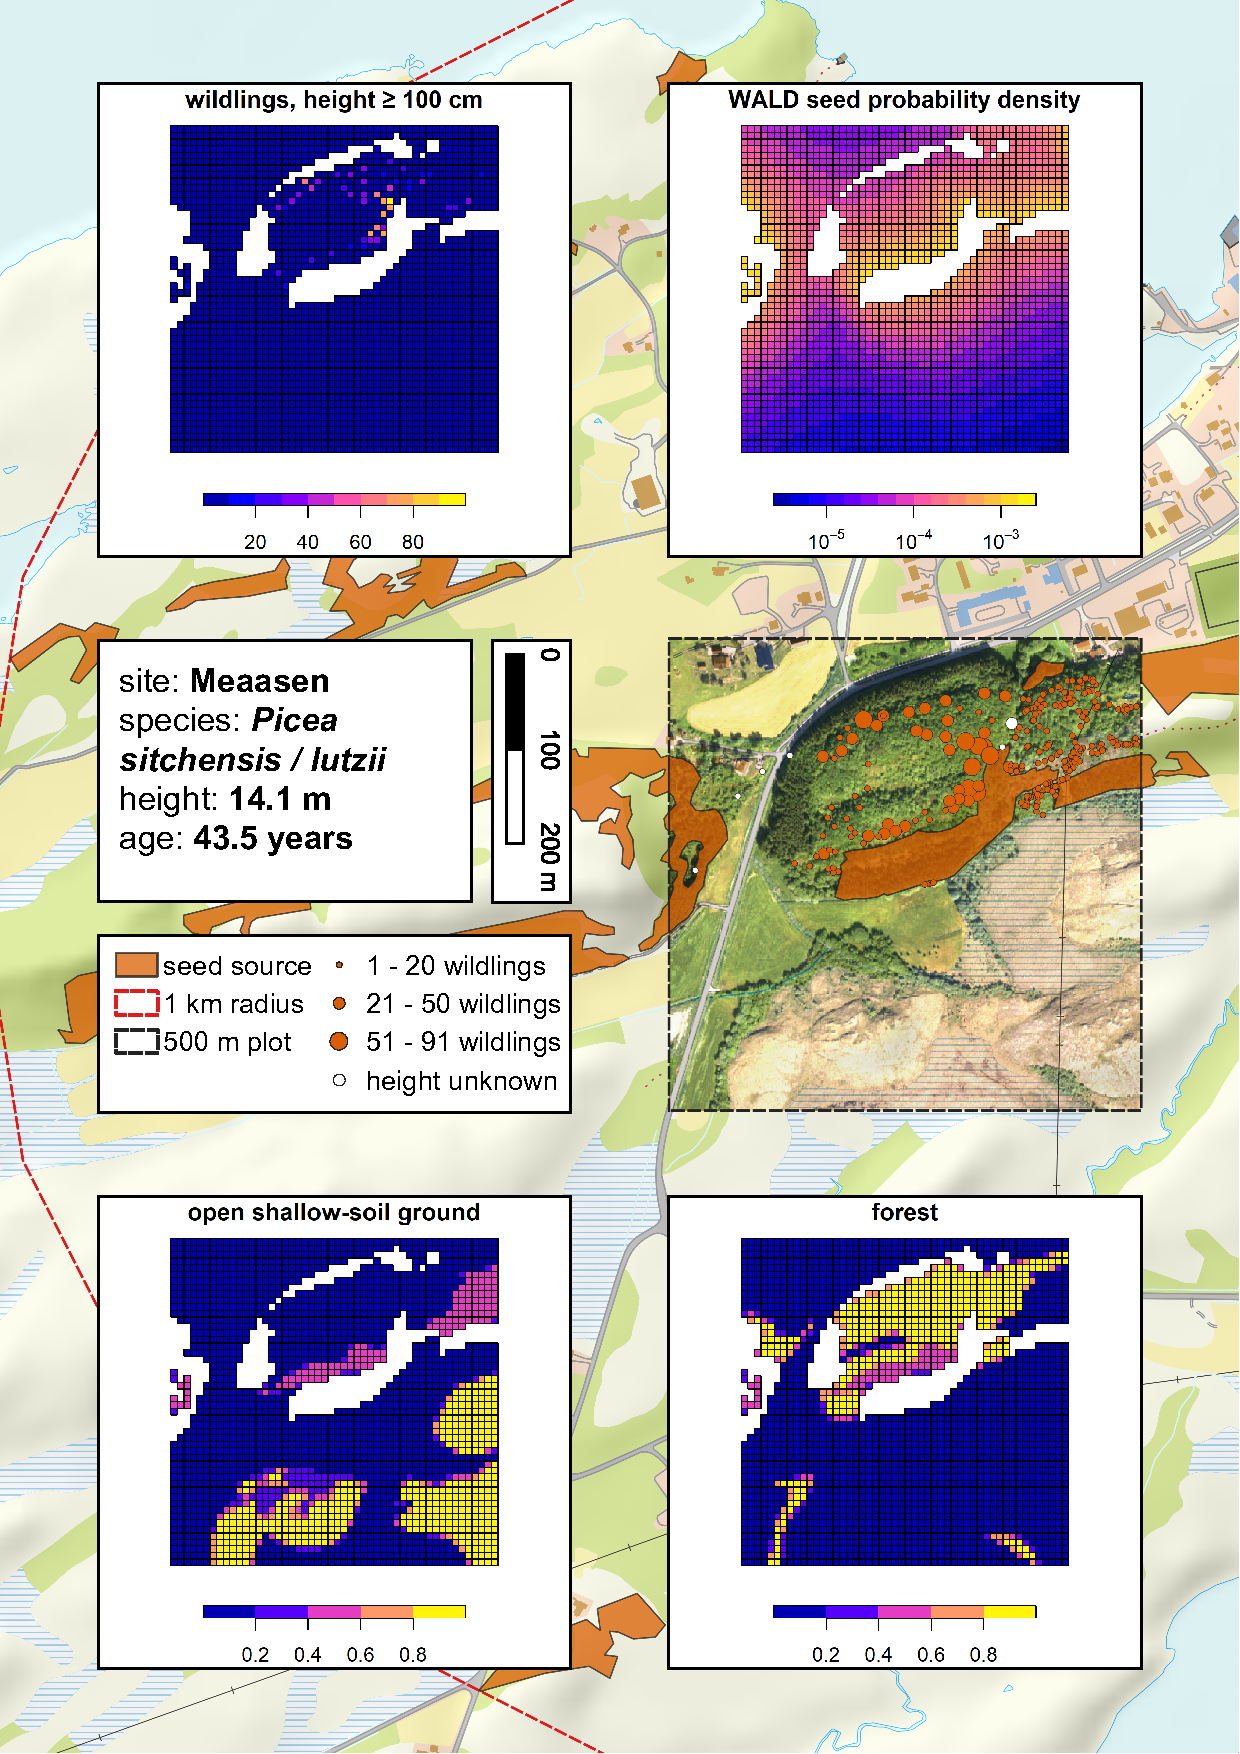
\includegraphics[width=0.9\linewidth]{figures/site-example/site-example} \caption{An illustration of one of the 76 plantations: Meaasen. The background map shows the surroundings of the plantation, and the 500x500 m plot is overlaid with an aerial photograph. The middle row of panels shows data as registered in the field. The top and bottom rows of panels show selected variables for the 500x500 m plot, as used in the regression model (with a spatial grain of 10 m). Grid cells without data are either seed sources or "tree plantations" of other species.}\label{fig:site-example}
\end{figure}

We used a directed acyclic graph (DAG) to diagram causal relationships among the
factors we expected to influence wildling abundance per cell
(fig.~\ref{fig:DAG}). In the DAG, the unmeasured, proximate causes of wildling
abundance --- total seed rain over the lifetime of the stand and establishment
likelihood --- are descendants of variables that we could observe or model. We
included an effect of elevation relative to the stand on seed rain because
neither of our models of seed dispersal account for uneven terrain.

\begin{figure}
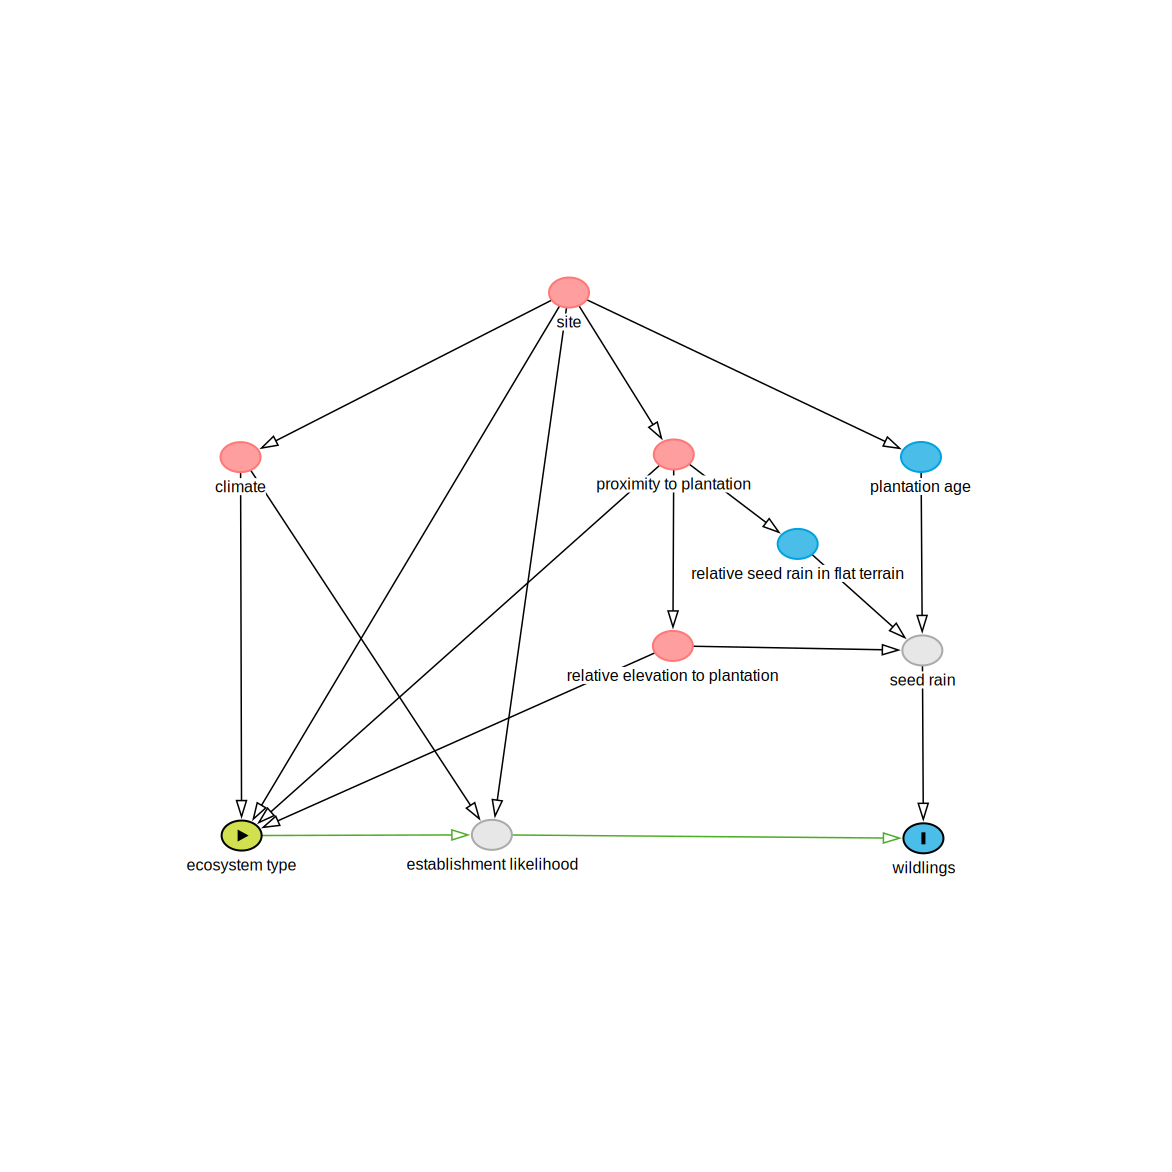
\includegraphics[width=0.9\linewidth]{figures/dagitty-model} \caption{A directed acyclic graph showing the assumed causal relationships motivating our statistical model of ecosystems' effects on wildling abundance. Red variables causally affect both the ecosystem type and wildling abundance, blue variables causally affect only wildling abundance, and grey variables are unobserved. Green arrows show the causal pathway of interest.}\label{fig:DAG}
\end{figure}

For all species, wildling abundance showed a high frequency of zeros that was
underestimated by the best fitting negative binomial distribution. Accordingly,
we applied zero-inflated generalized linear models, fitted with the glmmTMB
package (version 1.0, \citeproc{ref-brooksGlmmTMBBalancesSpeed2017}{Brooks et al., 2017}) in R (version 3.6, \citeproc{ref-rcoreteamLanguageEnvironmentStatistical2020}{R Core Team, 2020}). These zero-inflated models regard
zeros as the mixed product of a binomial process as well as a (conditional)
count process that can take different error distributions
(\citeproc{ref-zuurMixedEffectsModels2009}{Zuur et al., 2009}). Preliminary models fitted with a negative
binomial error distribution in the count process (ZINB) sometimes showed
residual underdispersion, so we switched to a generalized Poisson error
distribution (ZIGP), which can accommodate both over- and underdispersion
(\citeproc{ref-brooksStatisticalModelingPatterns2019}{Brooks et al., 2019}).

We modeled the binomial process as dependent on stand age and site, with site as
a random variable. We expected that younger stands would exhibit more
wildling-free cells than predicted under a constant establishment rate from age
zero, because of their infertile juvenile period. We also expected the frequency
of zeros to vary with site, because our field work documented that some land
owners had occasionally made efforts to remove wildlings. Excess zeros that
arose in these ways would therefore not bias our estimates of establishment
likelihood (\citeproc{ref-blasco-morenoWhatDoesZero2019}{Blasco‐Moreno et al., 2019}).

To estimate the causal influence of ecosystems on wildling abundance in
accordance with the DAG (\citeproc{ref-mcelreathHauntedDAGCausal2020}{McElreath, 2020}; \citeproc{ref-textorRobustCausalInference2016}{Textor et al., 2016}), we modeled the count process as dependent on
ecosystem, site, climate, elevation relative to the stand, and relative seed
rain. We also included stand age in the count process model because it reduced
the unexplained variance associated with the random effect of site, and because
we could interpret its coefficient as an unconfounded total effect on wildling
abundance (\citeproc{ref-westreichTableFallacyPresenting2013}{Westreich \& Greenland, 2013}). Climate was represented as
mean annual temperature (Bio1) and precipitation of the coldest quarter (Bio19),
at 30~arcsecond resolution, from CHELSA data
(\citeproc{ref-kargerClimatologiesHighResolution2017}{Karger et al., 2017}). We chose these variables because they
showed the strongest correlations with Norwegian vegetation zones and sections,
respectively (\citeproc{ref-bakkestuenSteplessModelsRegional2008}{Bakkestuen et al., 2008}). Elevation relative to the
stand was taken with respect to the highest point of the central stand, from
digital elevation models at 1 or 10~m resolution (Norwegian Mapping Authority).
Relative seed rain directly represents relative exposure in the count process,
so we entered the natural log of this variable as an offset term {[}coefficient
fixed at 1; Zuur et al. (\citeproc{ref-zuurMixedEffectsModels2009}{2009}){]}. We expect, for example, that a
doubling in seed rain would result in a doubling in wildling abundance, all else
being equal.

To summarize, for each species we modeled:

\begin{equation}
\begin{aligned}
wildlings_{ij} &\sim ZIGP(\pi_{i}, \mu_{ij}, \phi) \\
logit(\pi_{i}) &= StandAge_{i} + Site_{i} \\
log(\mu_{ij}) &= \sum\limits_{k=1}^K EcosystemType_{ijk} + Site_{i} + Bio1_{i} + Bio19_{i} + \\
&RelativeElevation_{ij} + StandAge_{i} + \\
&offset(log(RelativeSeedRain_{ij})) \\
Site_{i} &\sim Normal(0, \sigma^2) \\
\end{aligned}
\end{equation}

where \(\pi\) is the probability of a zero from the binomial process, while \(\mu\)
and \(\phi\) are the mean and dispersion of the generalized Poisson distribution,
respectively (\citeproc{ref-brooksStatisticalModelingPatterns2019}{Brooks et al., 2019}). Subscripts \(i\), \(j\), and
\(k\) index sites, cells, and ecosystems.

For each species, wildling-free ecosystems were dropped as predictors (to avoid
model convergence issues stemming from complete separation), along with the
cells that were comprised mostly (\textgreater~0.5) of one of these ecosystems. The values
of Bio1, Bio19, elevation relative to the stand, and stand age were
standardized, and the natural log of relative seed rain was centered. We fitted
three parallel models for each species: (1) with relative seed rain derived from
the static dispersal kernel, (2) with relative seed rain derived from the WALD
dispersal model, and (3) without relative seed rain. From these three we
selected that with the best AIC. Three models (Sitka/Lutz spruce and Norway
spruce with static dispersal kernel; larches without seed rain) did not converge
and were excluded from selection. To catch problems with our model
specification, we looked for deviation from uniformity in quantile-scaled,
simulated residuals, using the DHARMa package (version 0.4.6, \citeproc{ref-hartigDHARMaResidualDiagnostics2020}{Hartig, 2020}). We also ran DHARMa's tests for residual
over/underdispersion and zero-inflation. Relative establishment likelihoods
among ecosystems were calculated as predictions from the conditional count part
of the model (holding covariates at their mean values).

To test whether higher-level characteristics of ecosystems can be used to
generalize patterns of susceptibility, we aggregated ecosystems by their
category (terrestrial or wetland) and structuring process (none, environmental
stress, regulating disturbance, destabilizing disturbance, moderate
anthropogenic disturbance, or strong anthropogenic disturbance), as defined in
the Nature in Norway system (Appendix, table~\ref{tab:types-table}). We then
refitted our selected models with these eight strata replacing ecosystems, and
obtained estimates of relative establishment likelihood for each category and
structuring process.

\section{Results}\label{results}

Wildling densities across ecosystems ranged 0-211/ha for Sitka/Lutz spruce
(unstratified mean: 28), 0-49/ha for Norway spruce (unstratified mean: 6), and
0-1045/ha for larches (unstratified mean: 13). Relative establishment
likelihoods differed considerably from relative wildling densities, except in
larches (table~\ref{tab:vul-sus-cor-table}). For instance, our model estimated
that Sitka/Lutz spruce is three times more likely to establish in ``boreal heath''
than in ``artificial substrate'', despite wildling density being three times lower
in ``boreal heath'' (fig.~\ref{fig:susceptibility-Ps}).

\begin{table}

\caption{\label{tab:vul-sus-cor-table}Correlations between vulnerability (surveyed) and susceptibility (modelled) across ecosystem types, for each species group and wildling class.}
\centering
\begin{tabular}[t]{>{}lrrr}
\toprule
species & hgtclass & pearson & spearman\\
\midrule
\em{Larix} & 2 & 0.9987682 & 0.8881119\\
\em{Larix} & NA & 0.9987866 & 0.8391608\\
\em{P.abies} & 2 & 0.4603591 & 0.9020979\\
\em{P.abies} & NA & 0.4154753 & 0.6789216\\
\em{P.sitchensis-lutzii} & 2 & -0.0542191 & 0.4590965\\
\addlinespace
\em{P.sitchensis-lutzii} & NA & 0.2711149 & 0.4055829\\
\bottomrule
\end{tabular}
\end{table}

For all species, models using relative seed rain estimates from the WALD
dispersal model predicted wildling abundance best (Appendix,
table~\ref{tab:dispersal-model-comparison-table}). Site had a strong influence
on wildling abundance for Sitka/Lutz spruce, such that site variation swamped
much of the variation between ecosystems for this species. The direct effects of
climate on establishment likelihood varied by species and was strongest for
larches (Appendix, tables~\ref{tab:PsNA}--\ref{tab:L2}). The direct effects of
elevation relative to the stand on wildling abundance were comparatively modest
and acted in different directions for different species. Stand age did not
significantly affect wildling abundance in any species, except that older stands
of Sitka/Lutz spruce had fewer wildling-free cells (structural zeros) than
younger stands.

\begin{figure}
\centering
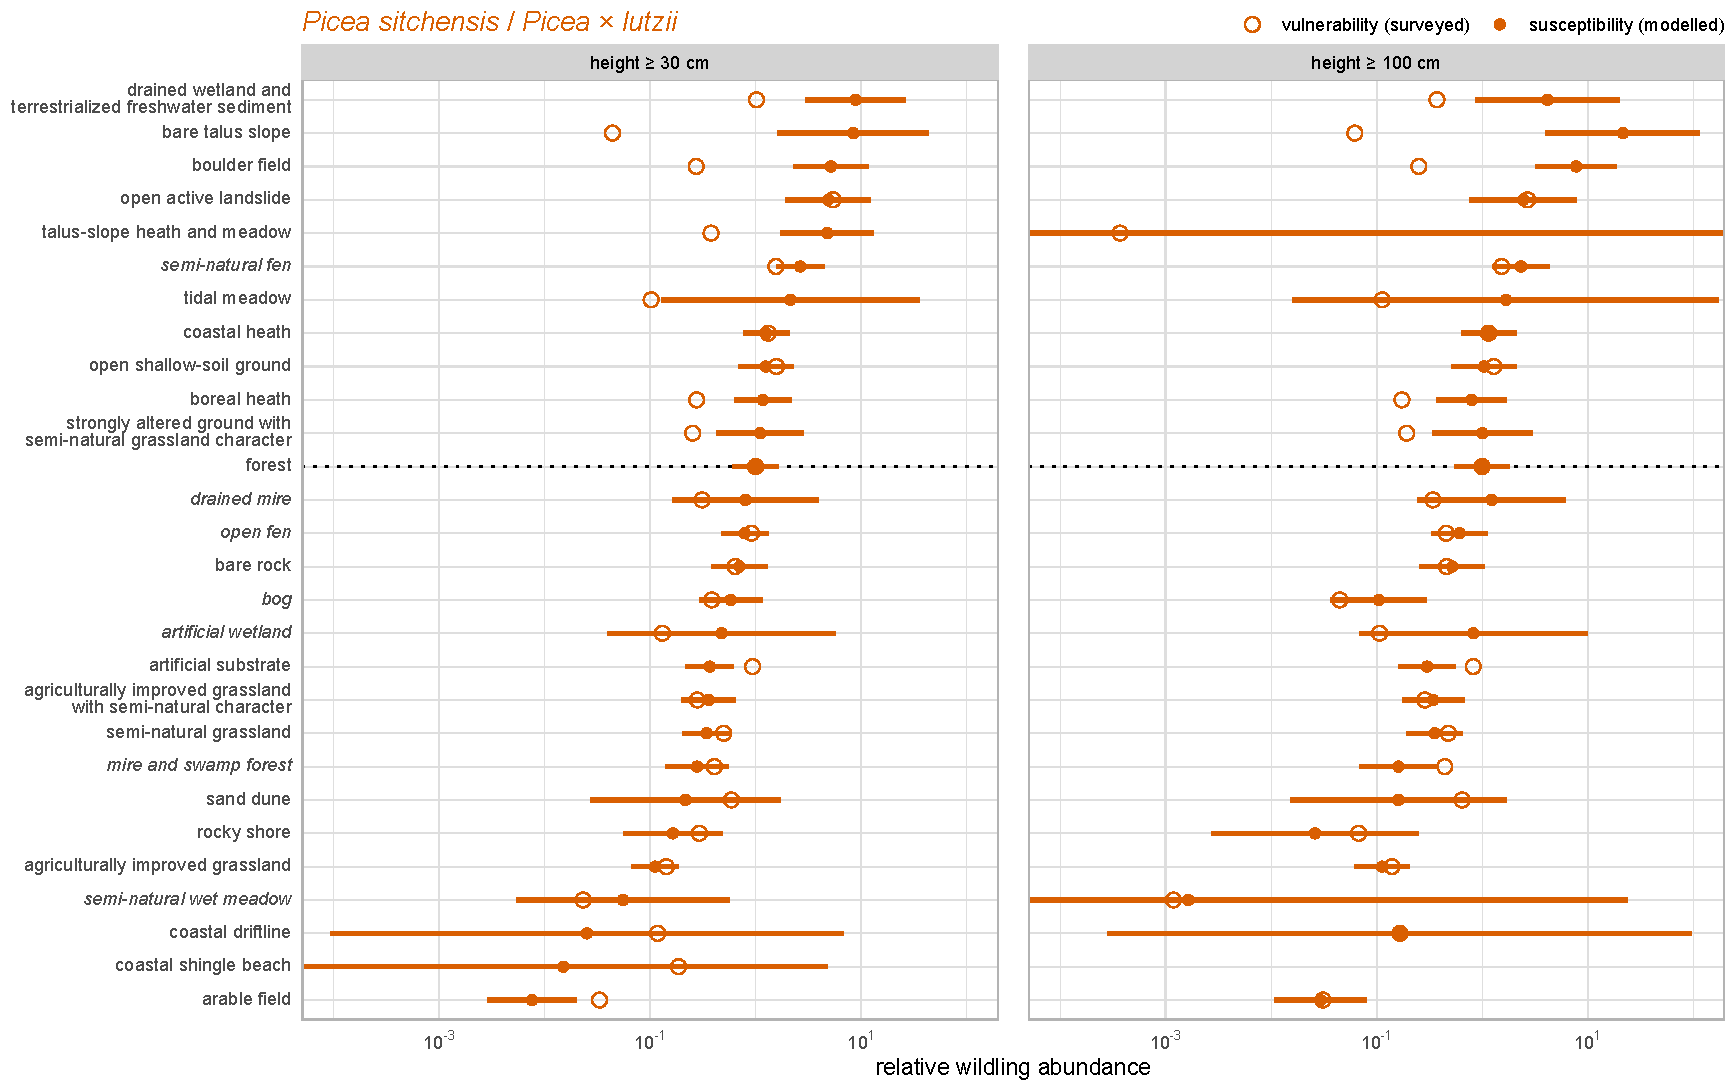
\includegraphics{figures/susceptibility/Ps.pdf}
\caption{\label{fig:susceptibility-Ps}Relative vulnerability (unfilled points) and susceptibility (filled points) of Picea sitchensis / Picea \times lutzii across ecosystem types, using `forest' as the reference ecosystem. Zero density is plotted at the lower limit of the x-axis. Relative establishment likelihoods are shown with 95 \% confidence intervals. The order of ecosystem types along the y-axis is by susceptibility to wildlings with height \(\geq\) 30 cm.}
\end{figure}

\begin{figure}
\centering
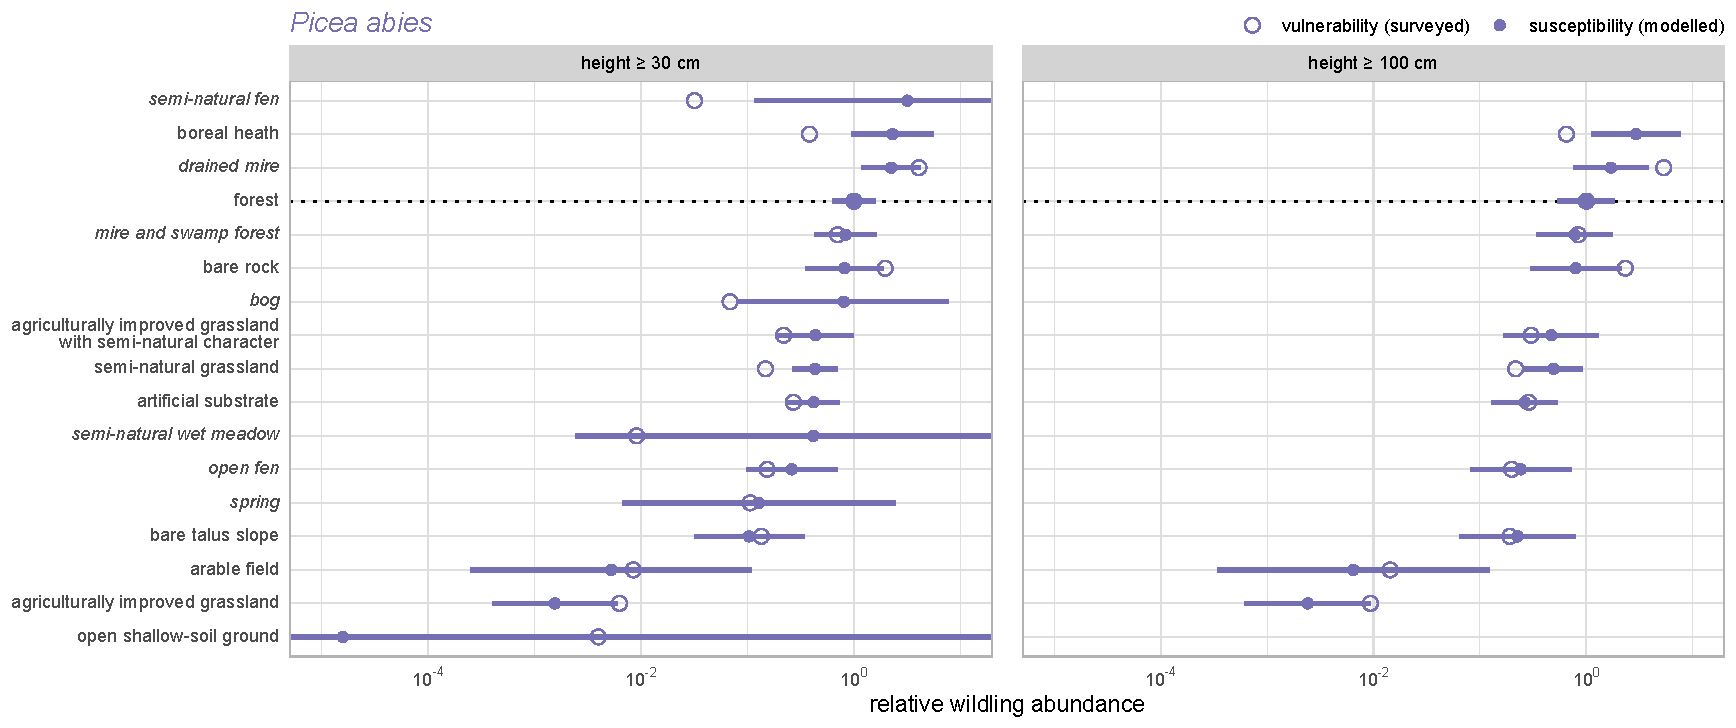
\includegraphics{figures/susceptibility/Pa.pdf}
\caption{\label{fig:susceptibility-Pa}Relative vulnerability (unfilled points) and susceptibility (filled points) of Picea abies across ecosystem types, using `forest' as the reference ecosystem. Zero density is plotted at the lower limit of the x-axis. Relative establishment likelihoods are shown with 95 \% confidence intervals. The order of ecosystem types along the y-axis is by susceptibility to wildlings with height \(\geq\) 30 cm.}
\end{figure}

\begin{figure}
\centering
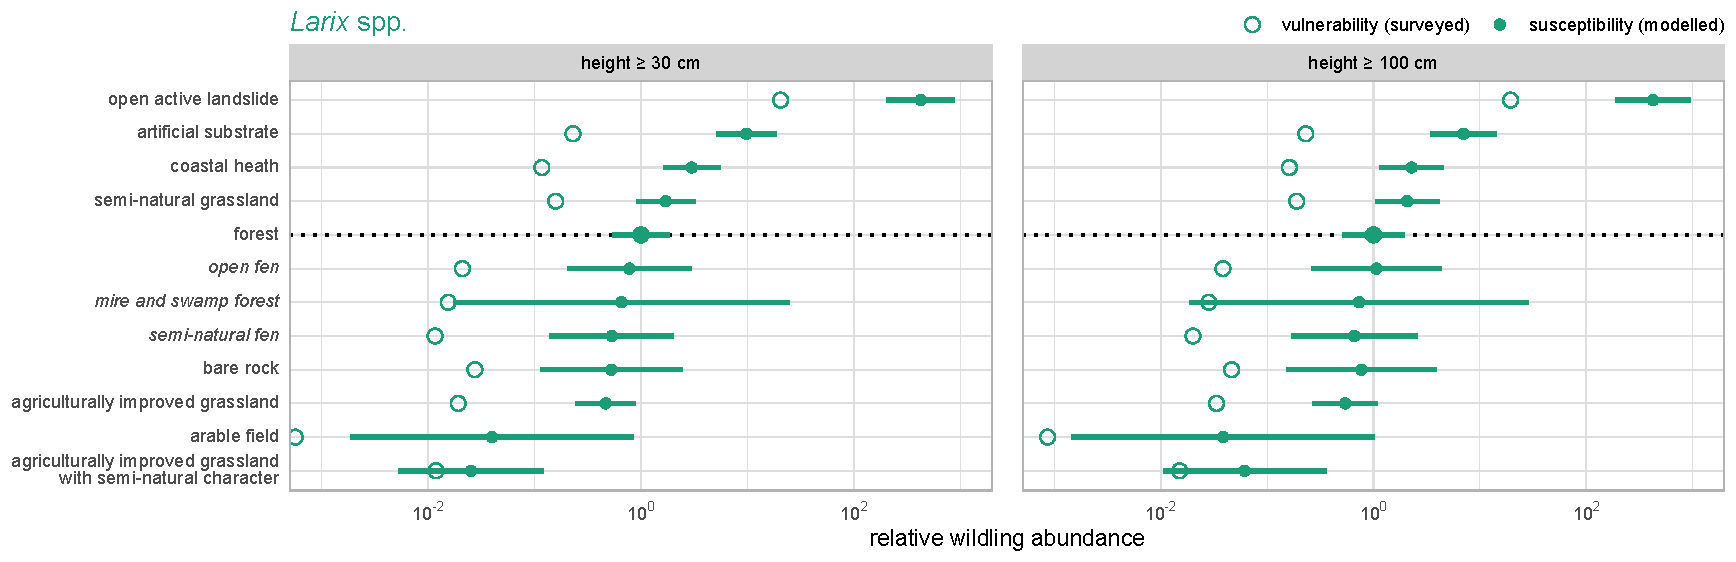
\includegraphics{figures/susceptibility/L.pdf}
\caption{\label{fig:susceptibility-L}Relative vulnerability (unfilled points) and susceptibility (filled points) of Larix spp. across ecosystem types, using `forest' as the reference ecosystem. Zero density is plotted at the lower limit of the x-axis. Relative establishment likelihoods are shown with 95 \% confidence intervals. The order of ecosystem types along the y-axis is by susceptibility to wildlings with height \(\geq\) 30 cm.}
\end{figure}

Among ecosystems with at least one wildling, estimated establishment likelihoods
varied by 3--5 orders of magnitude for the different species. Patterns of
relative establishment likelihood were modestly similar between species, with
positive rank correlations in four of six species pairs
(table~\ref{tab:species-correlation-table}). ``Arable fields'' showed some of the
lowest establishment likelihoods of any ecosystem for all species where it
appeared. Meanwhile, ecosystems with high establishment likelihoods tended to be
rarer types (e.g.~``open active landslides'') but also included ``boreal heath'' and
``coastal heath''.

\begin{table}

\caption{\label{tab:species-correlation-table}Correlations in susceptibility of ecosystem types between pairs of species groups, separately for each wildling class.}
\centering
\begin{tabular}[t]{rllrr}
\toprule
\em{hgtclass} & \em{species1} & \em{species2} & \em{pearson} & \em{spearman}\\
\midrule
2 & P.sitchensis-lutzii & P.abies & -0.1539583 & 0.5104895\\
2 & P.sitchensis-lutzii & Larix & 0.6360925 & 0.5594406\\
2 & P.abies & Larix & -0.1047041 & 0.2833333\\
NA & P.sitchensis-lutzii & P.abies & 0.0380192 & 0.3176471\\
NA & P.sitchensis-lutzii & Larix & 0.8593768 & 0.5664336\\
\addlinespace
NA & P.abies & Larix & -0.1124636 & 0.1757576\\
\bottomrule
\end{tabular}
\end{table}

Variation in establishment likelihoods shrank when ecosystems were aggregated by
category or structuring process, to 0--3 orders of magnitude. None of the
species showed large differences in establishment likelihood between terrestrial
and wetland ecosystems. At most, larches were three times less likely to
establish in wetlands. Ecosystems structured by destabilizing disturbance tended
to show high establishment likelihoods. However, the association between
structuring process and establishment likelihood was heterogeneous across
species.

\section{Discussion}\label{discussion}

\subsection{How does wildling density relate to ecosystem susceptibility?}\label{how-does-wildling-density-relate-to-ecosystem-susceptibility}

Confounders of the relationship between ecosystem type and wildling density
caused density to mischaracterize differences in establishment likelihood
between ecosystems. For example, the density of Sitka/Lutz spruce wildlings was
about equal in ``bare talus slopes'' and ``arable fields'', but we estimate that
establishment likelihood is actually about 1000 times higher in the former. The
nonzero effects of hypothesized confounders (like seed rain, climate, and site)
imply that our modeled estimates of establishment likelihood are less biased
measures of ecosystem susceptibility. Furthermore, variation in establishment
likelihood was no smaller than variation in wildling densities, as might have
been the case if confounding variables had amplified differences in ecosystem
establishment.

Because wildling abundance is the product of seed rain and establishment
likelihood, we needed to estimate seed rain independently of our wildling data
to model establishment likelihood properly. By including relative seed rain as
an offset in the model, we ensured that seed rain and establishment likelihood
were not conflated, at the cost of assuming that our relative seed rain
estimates were accurate. Exploring the alternative, we found that if we included
relative seed rain as a covariate rather than an offset that its coefficient was
estimated near one, and that estimated relative establishment likelihoods
remained mostly unchanged (Appendix, fig.~\ref{fig:sensitivity-offset}).
Although wildlings cannot rigorously validate seed dispersal models (due to
survivorship bias), the superior fits of models with WALD-derived seed rain
offsets compared to models with statically-derived seed rain offsets supports
the WALD model estimates. The mechanistic nature of the WALD model also makes us
more confident in its estimates across species and sites than we would be in a
purely phenomenological model (\citeproc{ref-bullockAllDispersalFunctions2018}{Bullock et al., 2018}). Nevertheless,
that seed rain was modeled and not measured is a limitation of our method, and
it makes the establishment likelihoods we estimate less certain. For example,
changes in the distribution of seed rain as a stand matures were not accounted
for, nor was secondary seed dispersal from the few reproductive wildlings we
observed.

The inconsistent effects of relative elevation on wildling abundance indicate
that there is no rule of thumb for management about wildlings moving up or down
slopes. However, since we defined elevation relative to the central stand, it is
possible that seed sources above or below the central stand partly masked slope
effects. On the other hand, our results were consistent with the idea that
prevailing winds during the dispersal season affect the direction of wildling
spread, since the WALD model provided the best fit. Meanwhile, the weak and
uncertain effects of stand age on wildling abundance suggests that other site
characteristics tend to outweigh the magnitude of wildling accumulation over
time.

Our models do not estimate climate's total causal effect on wildling abundance,
because they set aside its influence on ecosystems
(\citeproc{ref-westreichTableFallacyPresenting2013}{Westreich \& Greenland, 2013}). Therefore, we interpret the estimated
climatic effects with respect to physiological constraints within a given
ecosystem. The negligible effect of precipitation and weakly positive effect of
mean annual temperature on Sitka/Lutz spruce wildling abundance is consistent
with Sitka spruce's wide climatic tolerance relative to climatic variation in
Norway and its oceanic affinity (\citeproc{ref-petersonEcologyManagementSitka1997}{Peterson et al., 1997}). For
Norway spruce, our results support a previous finding that seedling recruitment
increases towards the wetter end of Norwegian climate
(\citeproc{ref-tingstadTemperaturePrecipitationBiotic2015}{Tingstad et al., 2015}), although most of our sites
circumscribed a narrow part of that range. Warm and wet conditions seem to
suppress larch establishment in Norway, which may be taken into consideration
when managing these plantations.

A curious feature of our results that needs more research is the large amount of
unexplained variation in Sitka/Lutz spruce wildling abundance between sites.
This means that our ability to predict the spread of this species at a specific
site, relative to others, is limited. Nevertheless, ecosystem comparisons can
and should still guide management. Bianchi et al.
(\citeproc{ref-bianchiMethodsPredictingSitka2019}{2019}) struggled to predict regeneration density
within Sitka spruce plantations from stand density (among other predictors),
which suggests that the unexplained site-level variation in our models was not
caused by our assumption of constant seed source density. Alternative sources of
heterogeneity may include: (1) disturbance legacies not captured in the
delineation of ecosystem types {[}especially in grazing pressure;
Miller et al. (\citeproc{ref-millerHowDisturbanceHistory2021}{2021}){]}, (2) demographic characteristics of
plantations, potentially related to provenance {[}especially in cone production;
Taylor et al. (\citeproc{ref-taylorDriversPlantInvasion2016}{2016}){]}, (3) wildling control by property owners, or
(4) ecological differences between Sitka and Lutz spruce.

\subsection{Which ecosystems are susceptible?}\label{which-ecosystems-are-susceptible}

In a large database of vegetation plots across Europe, Chytrý et
al.(\citeproc{ref-chytryHabitatInvasionsAlien2008}{2008}) found that alien plants as a group are
consistently found at low rates in mires and heaths, and high rates in arable,
man-made, and coastal ecosystems. The conifer species we examined do not conform
closely to these broader trends in ecosystem invasibility, showing relatively
high rates of establishment in heaths and very low rates of establishment in
arable ecosystems. To the extent that there are similarities across these four
species, they appear to establish more easily in ecosystems infrequently hit by
intense disturbances (e.g.~rock fall in ``bare talus slope'') than in ecosystems
frequently experiencing less intense disturbances (e.g.~flooding in
``semi-natural wet meadow'').

It is difficult to evaluate our results against the recruitment patterns that
have been described for the three species. For instance, Sitka spruce grows
poorly under moisture stress and tolerates flooding well
(\citeproc{ref-petersonEcologyManagementSitka1997}{Peterson et al., 1997}), which might account for why it was
equally likely to establish in wetland and terrestrial ecosystems. Yet it also
established well in ``open shallow-soil ground'', despite this ecosystem's
characteristically dry soil. This illustrates the trouble with deriving
predictions from generalized statements about species autecology. Furthermore,
ecosystems that would seem inhospitable based on their overall characteristics
may actually contain many localized opportunities for establishment, because
seedling mortality is strongly regulated by microsites
(\citeproc{ref-macekLifeDeathPicea2017}{Macek et al., 2017}). From this perspective, our estimates of
establishment likelihood measure the density of suitable microsites in a given
ecosystem.

The breadth in establishment likelihood suggests that differences between
ecosystems deserve careful consideration when managing wildling spread. This
knowledge may be applied in at least two ways. First, as a preventative measure,
we recommend siting new stands where surrounded by high proportions of
ecosystems with low establishment likelihood. In particular, ``arable fields''
repress wildling establishment for all species and are common near existing
stands, so picking sites hemmed in by this kind of agricultural land should be
both effective and feasible. This would probably reduce the rate of wildling
establishment by orders of magnitude, even if long distance dispersal might
preclude complete containment (\citeproc{ref-albertLanduseChangeSubalpine2008}{Albert et al., 2008}). In some cases
it may also be desirable to transform ecosystems adjacent to existing stands to
prevent (further) spread, for example by intensifying mowing regimes. Second, as
a reactive measure, we advise using relative ecosystem susceptibility as a
starting point for allocating monitoring and control resources in proportion to
risk. Prioritizing ecosystems that are highly susceptible and also rare (e.g.
``open active landslide'') is especially likely to be cost-efficient.

The establishment patterns we quantify probably hold, more or less, outside
Norway (\citeproc{ref-chytryHabitatInvasionsAlien2008}{Chytrý, Maskell, et al., 2008}). From a manager's perspective, we
expect that the ecosystems we report may translate well to equivalent types in
similar classification systems, because the Nature in Norway classification is
rule-based and aims for observer neutrality. At the same time, we urge caution
in extending our establishment estimates to ecosystems that are only broadly
similar, because similar types frequently showed markedly different
susceptibility (e.g.~Norway spruce in ``agriculturally improved grassland with
semi-natural character'' vs.~``agriculturally improved grassland'').

An observational study like ours informs management of long-lived, naturalized
species more directly than experimental studies, because longer time frames are
examined. It measures long-term survival under a wide range of natural
conditions experienced by the wildlings. In contrast, seeding experiments
generally observe only the youngest life stages, and the factors controlling
individual success differ at later life stages
(\citeproc{ref-dovciakSeedRainEnvironmental2008}{Dovčiak et al., 2008}). On the other hand, experiments might be
more useful when the observed wildling spread is not broadly representative
(e.g.~for species expanding from a single, recent introduction).

\subsection{What do susceptible ecosystems have in common?}\label{what-do-susceptible-ecosystems-have-in-common}

The overarching characteristics that we used to aggregate ecosystems did not
generalize differences in susceptibility well, especially not across species, so
these classifications have limited utility for management. Note that different
sets of ecosystems comprised the strata for each species, depending on their
presence in the data, and these differences in ecosystem composition help
explain why the patterns of aggregated establishment likelihood varied between
species. This constraint hinders species comparisons but underlines our main
takeaway from these results --- that the susceptibility of an individual
ecosystem frequently diverges from those of related ecosystems.

Within species, we urge careful interpretation of the comparisons among
ecosystem categories and structuring processes. Many areas where conifer
establishment is nearly impossible, like paved surfaces and annually plowed
fields, count as terrestrial and strongly anthropogenically disturbed, which
lowers the relative establishment likelihood of these two strata. Our results do
not imply, for example, that a strong anthropogenic disturbance event will
decrease establishment likelihood of Sitka/Lutz spruce relative to an
ecosystem's prior state. Rather, we find that ecosystems structured by strong
anthropogenic disturbance, on the whole, are less susceptible to Sitka/Lutz
spruce wildlings than other ecosystems.

\section{Conclusions}\label{conclusions}

One of the main novelties of this study is that we inferred
susceptibility/invasibility using mechanistically reconstructed, spatial
estimates of seed rain. Scientists studying invasibility at national and
continental scales have already recognized the importance of normalizing
observed levels of invasion by a spatially explicit estimate of exposure {[}i.e.
propagule pressure; Colautti et al. (\citeproc{ref-colauttiPropagulePressureNull2006}{2006});
Chytrý, Jarošík, et al. (\citeproc{ref-chytrySeparatingHabitatInvasibility2008}{2008}){]}. However, many studies quantifying
ecosystem invasibility have not been able to adjust for propagule pressure,
typically because it is impossible to reconstruct the underlying dispersal
history (\citeproc{ref-catfordQuantifyingLevelsBiological2012}{Catford et al., 2012}). We found that accounting for
seed rain and other confounders of the relationship between ecosystems and
wildling abundance reshuffles estimates of ecosystem invasibility considerably.

Wildling spread from plantations is a growing problem
(\citeproc{ref-richardsonConifersInvasiveAliens2004}{Richardson \& Rejmánek, 2004}) and will probably worsen with recent
pushes to increase tree planting worldwide
(\citeproc{ref-brunduGlobalGuidelinesSustainable2020}{Brundu et al., 2020}). Meanwhile, remotely sensed and
surveyed data are increasing the availability of detailed and accurate maps of
ecosystems across large areas, which presents opportunities to manage wildling
spread more efficiently. Specifically, differences in ecosystem susceptibility
may be leveraged to reduce the rate of wildling establishment through deliberate
site selection for new stands or targeted interventions around existing stands.
However, managers should not judge ecosystem susceptibility based on wildling
density alone, nor on generalizations across ecosystems.

\section{Authors' contributions}\label{authors-contributions}

JV, SLO, and OSk conceived the study and designed the methodology; SLO, LA, MOK,
AO, JS, OSt, and ØS collected the data; JV analyzed the data and led the
writing. All authors contributed to drafts and gave approval for publication.

\section{Acknowledgments}\label{acknowledgments}

We thank Ola Westby Aamodt, Matteo De Stefano, Vigdis Frivoll, Honorata Gajda,
Miene-Marie Gastinger, Jon Hagelin, Craig Jackson, Roy Mangersnes, Heidi Elin
Myklebost, Bjarne Homnes Oddane, Sina Thu Randulff, Anders Ringstad, Monica
Ruano, Knut Børge Strøm, Rune Søyland, Solbjørg Engen Torvik, and Toralf Tysse
for their help in collecting and/or collating the field data. Field work was
financed by the Norwegian Environment Agency (contracts 15040036, 17070025,
17070031, 19087470, 19087471).

\section{Data availability statement}\label{data-availability-statement}

Data will be made available via the Dryad Digital Repository. Code is available
at \url{https://github.com/julienvollering/conifer-plantation-spread}.

\newpage

\section{Appendix}\label{appendix}

The WALD model (\citeproc{ref-katulMechanisticAnalyticalModels2005}{Katul et al., 2005}) takes the form of an
inverse Gaussian distribution whose mean (\(\mu\)) and shape (\(\lambda\))
parameters are calculated from physical characteristics of the dispersal system:

\begin{equation}
\mu = \frac{HU}{F}
\end{equation} \begin{equation}
\lambda = \left(\frac{H}{\sigma}\right)^2
\end{equation}

where \(H\) is the seed release height, \(U\) is the mean horizontal wind velocity
between \(H\) and the ground, \(F\) is the terminal velocity of the seed, and
\(\sigma\) is a wind turbulence parameter. We set \(H\) to the height of the central
stand, estimated \(U\) from a computed vertical wind profile, obtained \(F\) from
literature, and calculated \(\sigma\) from an equation for turbulent flow as a
function of vegetation height (eq. A4 in \citeproc{ref-skarpaasDispersalPatternsDispersal2007}{Skarpaas \& Shea, 2007}). We parameterized separate WALD models
for 20º sectors around each seed source, to make seed dispersal anisotropic
(directional). In each sector we estimated mean vegetation height based on the
composition of mapped ecosystem types (Appendix, table~\ref{tab:types-table}).
Simultaneously, we randomly sampled 100 wind velocities in the direction of the
sector during the species' dispersal season. The 100 resulting WALD kernels
produced the seed probability density in the sector, and individual sectors were
weighed by the frequency of corresponding wind directions (again, during the
species' dispersal season). The wind data were obtained either from the nearest
weather station (MET Norway), a 2.5 km resolution interpolated hindcast covering
southern Norway (\citeproc{ref-haakenstad15yearHighResolution2017}{Haakenstad \& Haugen, 2017}), or a 10 km resolution
hindcast covering all of Norway (\citeproc{ref-haakenstadNORA10EIRevisedRegional2020}{Haakenstad et al., 2020}; \citeproc{ref-reistadHighresolutionHindcastWind2011}{Reistad et al., 2011}). We used weather station data if the
station was less than 2.5 or 10 km away (depending on hindcast coverage), or
else the highest resolution hindcast.

\newpage

\begin{ThreePartTable}
\begin{TableNotes}
\item \textit{References: } 
\item 1. Harris, A. S. Sitka spruce. in Silvics of North America: 1. Conifers (eds. Burns, R. M. \& Honkala, B. H.) vol. 2 513–529 (U.S. Department of Agriculture, Forest Service, 1990).
\item 2. Sullivan, J. Picea abies. Fire Effects Information System, U.S. Department of Agriculture, Forest Service, Rocky Mountain Research Station,  Fire Sciences Laboratory https://www.fs.usda.gov/database/feis/plants/tree/picabi/all.html (1994).
\item[1] 3. Sullivan, J. Larix decidua. Fire Effects Information System, U.S. Department of Agriculture, Forest Service, Rocky Mountain Research Station,  Fire Sciences Laboratory https://www.fs.usda.gov/database/feis/plants/tree/lardec/all.html (1994).
\item[a] 4. Sandvik, H. Kunnskapsstatus for spredning og effekter av fremmede bartrær på biologisk mangfold. (2012).
\end{TableNotes}
\begin{longtable}[t]{>{}llll}
\caption{\label{tab:traits-table}Dispersal traits}\\
\toprule
species group & seed terminal velocity & dispersal season & references\\
\midrule
\em{Picea sitchensis / Picea \times lutzii} & 0.94 m/s & Oct - Feb & 1, 4\\
\em{Picea abies} & 0.58 m/s & Nov - May & 2, 4\\
\em{Larix spp.} & 1.0 m/s & Dec - May & 3, 4\\
\bottomrule
\insertTableNotes
\end{longtable}
\end{ThreePartTable}

Some of the seed source polygons we registered in the field had distinctive
features that we accounted for as follows. Seed source polygons for which the
species of interest only made up a fraction of the stand composition (e.g.~in \citeproc{ref-olsenKartleggingAvKortdistansespredning2019}{Olsen et al., 2019}) were used with their point source
density adjusted accordingly. For example, a stand identified as composed of
Sitka spruce and Norway spruce was assigned a seed source point density half
that of a Sitka spruce monoculture. Likewise, `mixed forest' stands (e.g.~in \citeproc{ref-appelgrenKartleggingAvKortdistansespredning2018}{Appelgren, 2018}) were assigned 0.1 times the
seed source point density of a monoculture. Seed source polygons identified as
logged (e.g.~in \citeproc{ref-appelgrenKartleggingAvKortdistansespredning2018}{Appelgren, 2018}) were included
as seed sources only if we could confirm that they were logged no earlier the
decade prior to mapping, using time series of aerial photos.

\begin{landscape}
\begin{longtable}[t]{lllllllll}
\caption{\label{tab:sites-table}\label{tab:sites-table}Plantation stands}\\
\toprule
reference & species group & site & easting & northing & height & age & bio01\textsuperscript{a} & bio19\textsuperscript{b}\\
\midrule
\endfirsthead
\caption[]{\label{tab:sites-table}Plantation stands \textit{(continued)}}\\
\toprule
reference & species group & site & easting & northing & height & age & bio01\textsuperscript{a} & bio19\textsuperscript{b}\\
\midrule
\endhead

\endfoot
\bottomrule
\multicolumn{9}{l}{\rule{0pt}{1em}\textit{Note: }}\\
\multicolumn{9}{l}{\rule{0pt}{1em}Easting and Northing are given for UTM zone 33N. Height is given in meters and age in years.}\\
\multicolumn{9}{l}{\rule{0pt}{1em}\textsuperscript{a} mean annual temperature (°C)}\\
\multicolumn{9}{l}{\rule{0pt}{1em}\textsuperscript{b} precipitation in coldest quarter (cm)}\\
\multicolumn{9}{l}{\rule{0pt}{1em}\textsuperscript{*} interpolated as the mean height of conspecific stands, inversely weighted by difference in age}\\
\multicolumn{9}{l}{\rule{0pt}{1em}\textsuperscript{\dag} interpolated as the mean age of conspecific stands in the same region}\\
\endlastfoot
Olsen et al. 2016 & Picea sitchensis / P. \times lutzii & Gryttingdalen-vest & 503887 & 7613803 & 8 & 52 & 4.56 & 49.0\\
Olsen et al. 2016 & Picea sitchensis / P. \times lutzii & Gryttingdalen-oest & 504335 & 7613736 & 8 & 52 & 4.50 & 50.5\\
Olsen et al. 2016 & Picea sitchensis / P. \times lutzii & Holmsnes-nordvest & 493935 & 7609464 & 11 & 49 & 5.36 & 45.3\\
Olsen et al. 2016 & Picea sitchensis / P. \times lutzii & Holmsnes-soeroest & 494675 & 7608420 & 11 & 45 & 5.46 & 44.0\\
Olsen et al. 2016 & Picea sitchensis / P. \times lutzii & Hov & 496920 & 7608739 & 11 & 56 & 5.22 & 50.9\\
\addlinespace
Olsen et al. 2016 & Picea sitchensis / P. \times lutzii & Raavollmarka & 499105 & 7608885 & 18 & 59 & 4.80 & 51.1\\
Appelgren and Torvik 2017 & Larix spp. & Anisdal & -36439 & 6529890 & 22 & 56 & 7.37 & 38.8\\
Appelgren and Torvik 2017 & Larix spp. & Haalandsbotn & -37108 & 6532830 & 20 & 57.5 & 7.00 & 38.9\\
Appelgren and Torvik 2017 & Larix spp. & Roeynaasen & -31279 & 6547997 & 25 & 77.5 & 6.88 & 36.5\\
Appelgren and Torvik 2017 & Larix spp. & Storemo & -107 & 6588189 & 23 & 60 & 7.15 & 33.0\\
\addlinespace
Appelgren and Torvik 2017 & Larix spp. & Toegjefjellet & -22293 & 6546411 & 20 & 60 & 6.69 & 39.6\\
Appelgren and Torvik 2017 & Larix spp. & Voren & -26899 & 6554824 & 20 & 62 & 6.42 & 39.6\\
Appelgren and Torvik 2017 & Picea abies & Mysingveien & -10547 & 6522150 & 21 & 52 & 6.34 & 53.9\\
Appelgren and Torvik 2017 & Picea abies & Ollestad & -2440 & 6519912 & 20\textsuperscript{*} & 58 & 6.76 & 42.5\\
Appelgren and Torvik 2017 & Picea abies & Varland & -15600 & 6584801 & 22 & 60 & 6.94 & 36.2\\
\addlinespace
Appelgren and Torvik 2017 & Picea sitchensis / P. \times lutzii & Dale & -30398 & 6586913 & 25 & 77 & 7.10 & 40.6\\
Appelgren and Torvik 2017 & Picea sitchensis / P. \times lutzii & Fjoesne & -11052 & 6650525 & 22 & 50 & 6.11 & 60.1\\
Appelgren and Torvik 2017 & Picea sitchensis / P. \times lutzii & Kvia & -42603 & 6539369 & 20 & 57.5 & 8.02 & 30.6\\
Appelgren and Torvik 2017 & Picea sitchensis / P. \times lutzii & Roeynaasen & -31321 & 6548005 & 23 & 77.5 & 6.88 & 36.5\\
Appelgren and Torvik 2017 & Picea sitchensis / P. \times lutzii & Toegjefjellet & -22347 & 6546467 & 20 & 60 & 6.69 & 39.6\\
\addlinespace
Appelgren and Torvik 2017 & Picea sitchensis / P. \times lutzii & Voren & -26991 & 6554850 & 18 & 52.5 & 6.42 & 39.6\\
Appelgren and Torvik 2017 & Picea sitchensis / P. \times lutzii & Aarheia & -33443 & 6589861 & 28 & 60 & 7.31 & 38.2\\
Kyrkjeeide et al. 2017 & Picea abies & Myklebostad & 481205 & 7469940 & 20\textsuperscript{*} & 97 & 4.99 & 24.9\\
Kyrkjeeide et al. 2017 & Picea abies & Tennes & 668660 & 7695332 & 20\textsuperscript{*} & 87 & 1.87 & 18.6\\
Kyrkjeeide et al. 2017 & Picea sitchensis / P. \times lutzii & Hagheia & 445925 & 7560670 & 18\textsuperscript{*} & 55 & 4.89 & 49.4\\
\addlinespace
Kyrkjeeide et al. 2017 & Picea sitchensis / P. \times lutzii & Harteigen & 449285 & 7559665 & 15\textsuperscript{*} & 51.5 & 5.38 & 48.4\\
Kyrkjeeide et al. 2017 & Picea sitchensis / P. \times lutzii & Haakoeya & 647074 & 7731726 & 17\textsuperscript{*} & 42\textsuperscript{\dag} & 3.16 & 30.0\\
Appelgren 2018 & Larix spp. & Engjane & -34540 & 6529860 & 15 & 45 & 7.19 & 40.3\\
Appelgren 2018 & Larix spp. & Hyljafjellet & -34030 & 6529963 & 15 & 45 & 7.30 & 39.6\\
Appelgren 2018 & Larix spp. & Hoegaas & -25415 & 6560056 & 20 & 57.5 & 6.77 & 38.8\\
\addlinespace
Appelgren 2018 & Larix spp. & Myrvoll & -12944 & 6522033 & 12 & 17.5 & 7.06 & 43.4\\
Appelgren 2018 & Larix spp. & Oaland & -7652 & 6563045 & 17 & 52.5 & 5.48 & 49.7\\
Appelgren 2018 & Picea abies & Efteland & -15304 & 6523548 & 20 & 45 & 6.69 & 53.8\\
Appelgren 2018 & Picea abies & Myrvoll & -13000 & 6522143 & 18 & 71.5 & 7.06 & 43.4\\
Appelgren 2018 & Picea sitchensis / P. \times lutzii & Foersvoll & -29434 & 6588711 & 24 & 54 & 7.22 & 37.7\\
\addlinespace
Appelgren 2018 & Picea sitchensis / P. \times lutzii & Hommeland & -17515 & 6559100 & 17 & 47 & 6.01 & 40.1\\
Appelgren 2018 & Picea sitchensis / P. \times lutzii & Hyljafjellet & -34044 & 6529954 & 13.5 & 45 & 7.30 & 39.6\\
Appelgren 2018 & Picea sitchensis / P. \times lutzii & Oaland & -7648 & 6563033 & 15 & 52.5 & 5.48 & 49.7\\
Appelgren 2018 & Picea sitchensis / P. \times lutzii & Sandve & -58701 & 6601600 & 11 & 30 & 7.83 & 38.8\\
Appelgren 2018 & Picea sitchensis / P. \times lutzii & Skorphella & -30767 & 6581293 & 13 & 35 & 7.87 & 31.3\\
\addlinespace
Appelgren 2018 & Picea sitchensis / P. \times lutzii & Starebakkane & -43287 & 6563381 & 18 & 52.5 & 8.08 & 27.9\\
Appelgren 2018 & Picea sitchensis / P. \times lutzii & Veggjaberget & -35788 & 6526000 & 12 & 27.5 & 8.04 & 35.0\\
Appelgren 2018 & Picea sitchensis / P. \times lutzii & Vikra & -59126 & 6601266 & 22\textsuperscript{*} & 78 & 7.97 & 37.5\\
Olsen et al. 2019 & Larix spp. & Stordalslia & 418827 & 7303180 & 11.9 & 16.5 & 4.62 & 52.2\\
Olsen et al. 2019 & Picea abies & Storbergan & 413255 & 7349964 & 13.1 & 49 & 5.02 & 55.6\\
\addlinespace
Olsen et al. 2019 & Picea abies & Svinnes & 385625 & 7306386 & 15.3 & 36.5 & 5.57 & 41.0\\
Olsen et al. 2019 & Picea sitchensis / P. \times lutzii & Alstahaugmyran & 382564 & 7311547 & 15.7 & 31.5 & 5.49 & 45.7\\
Olsen et al. 2019 & Picea sitchensis / P. \times lutzii & Hamran & 373448 & 7266074 & 17.2 & 26 & 5.69 & 42.3\\
Olsen et al. 2019 & Picea sitchensis / P. \times lutzii & Langvassfjellet & 409484 & 7330371 & 17.6 & 36.5 & 4.87 & 54.0\\
Olsen et al. 2019 & Picea sitchensis / P. \times lutzii & Meaasen & 386111 & 7333724 & 14.1 & 43.5 & 5.70 & 34.5\\
\addlinespace
Olsen et al. 2019 & Picea sitchensis / P. \times lutzii & Myrmo & 391075 & 7321058 & 18.8 & 37 & 5.22 & 37.4\\
Olsen et al. 2019 & Picea sitchensis / P. \times lutzii & Olabergan & 410600 & 7341996 & 18.8 & 29 & 5.31 & 45.0\\
Olsen et al. 2019 & Picea sitchensis / P. \times lutzii & Plogskjaeret & 378814 & 7280849 & 16.1 & 26 & 5.57 & 43.5\\
Olsen et al. 2019 & Picea sitchensis / P. \times lutzii & Sandmoan & 382107 & 7329122 & 10.8 & 33 & 5.73 & 33.7\\
Olsen et al. 2019 & Picea sitchensis / P. \times lutzii & Steinaasen & 375834 & 7274496 & 17.9 & 35 & 5.50 & 37.6\\
\addlinespace
Olsen et al. 2019 & Picea sitchensis / P. \times lutzii & Svinnes & 385652 & 7306426 & 16.4 & 37.5 & 5.65 & 40.1\\
Olsen et al. 2019 & Picea sitchensis / P. \times lutzii & Valan & 383545 & 7304119 & 15.5 & 35 & 5.61 & 41.5\\
Sandven et al. 2019 & Larix spp. & Ytre-bjotveit & 49799 & 6729344 & 19.4 & 72 & 5.52 & 34.5\\
Sandven et al. 2019 & Larix spp. & Knappeidet & -47542 & 6737678 & 17.2 & 32 & 7.99 & 39.4\\
Sandven et al. 2019 & Larix spp. & Indre-bjotveit & 51174 & 6730928 & 24.5 & 84 & 5.82 & 35.9\\
\addlinespace
Sandven et al. 2019 & Picea abies & Boerve & 37746 & 6711673 & 31.9 & 64 & 5.49 & 46.6\\
Sandven et al. 2019 & Picea abies & Skare & 31612 & 6676392 & 22 & 66 & 4.41 & 50.6\\
Sandven et al. 2019 & Picea abies & Oeystese & 16634 & 6726920 & 15.6 & 57 & 6.42 & 67.4\\
Sandven et al. 2019 & Picea abies & Vasshjallane & 65573 & 6728437 & 22.8 & 56 & 5.53 & 29.8\\
Sandven et al. 2019 & Picea abies & Hjelmtveit & -31407 & 6756542 & 21.4 & 57 & 7.15 & 57.3\\
\addlinespace
Sandven et al. 2019 & Picea abies & Bondhusdalen & 15726 & 6695404 & 16.2 & 55 & 5.67 & 44.0\\
Sandven et al. 2019 & Picea abies & Saeboe & -36690 & 6759365 & 21.2 & 51 & 7.07 & 59.8\\
Sandven et al. 2019 & Picea abies & Indre-arna & -25457 & 6738087 & 14.4 & 52 & 6.94 & 45.2\\
Sandven et al. 2019 & Picea abies & Kvamskogen & 4982 & 6726838 & 20.4 & 101 & 4.98 & 57.1\\
Sandven et al. 2019 & Picea abies & Rosendal & -1965 & 6685031 & 16.8 & 49 & 6.94 & 55.3\\
\addlinespace
Sandven et al. 2019 & Picea sitchensis / P. \times lutzii & Midtre-fjell & -47585 & 6729572 & 23.5 & 50 & 7.74 & 44.8\\
Sandven et al. 2019 & Picea sitchensis / P. \times lutzii & Oevre-manger & -43485 & 6764574 & 17.5 & 46 & 7.78 & 53.3\\
Sandven et al. 2019 & Picea sitchensis / P. \times lutzii & Fuglavasstoppen & -50243 & 6740596 & 19.5 & 48 & 7.86 & 46.0\\
Sandven et al. 2019 & Picea sitchensis / P. \times lutzii & Kvitefjella & -48847 & 6730154 & 21.1 & 50 & 7.57 & 47.6\\
Sandven et al. 2019 & Picea sitchensis / P. \times lutzii & Kausland & -50236 & 6718477 & 22.2 & 44 & 7.84 & 46.2\\
\addlinespace
Sandven et al. 2019 & Picea sitchensis / P. \times lutzii & Misje & -51009 & 6743828 & 20.8 & 54 & 7.99 & 45.1\\*
\end{longtable}
\end{landscape}

\begin{longtable}[t]{llr}
\caption{\label{tab:types-table}\label{tab:types-table}Ecosystem types, as defined by major types in the Nature in Norway system (codes). Approximate vegetation height (meters) is used only to parameterize wind turbulence for the WALD seed rain estimates.}\\
\toprule
type & code & vegetation height\textsuperscript{a}\\
\midrule
\endfirsthead
\caption[]{\label{tab:types-table}Ecosystem types, as defined by major types in the Nature in Norway system (codes). Approximate vegetation height (meters) is used only to parameterize wind turbulence for the WALD seed rain estimates. \textit{(continued)}}\\
\toprule
type & code & vegetation height\textsuperscript{a}\\
\midrule
\endhead

\endfoot
\bottomrule
\endlastfoot
bare rock & T1 & 0.0\\
open shallow-soil ground & T2 & 0.5\\
arctic-alpine heath and lee side & T3 & 0.5\\
forest & T4 & 10.0\\
rocky shore & T6 & 0.0\\
\addlinespace
tidal meadow & T12 & 0.5\\
bare talus slope & T13 & 0.0\\
talus-slope heath and meadow & T16 & 0.5\\
open active landslide & T17 & 0.0\\
open alluvial sediment & T18 & 0.0\\
\addlinespace
sand dune & T21 & 0.0\\
coastal driftline & T24 & 0.5\\
boulder field & T27 & 0.0\\
coastal shingle beach & T29 & 0.0\\
alluvial forest & T30 & 10.0\\
\addlinespace
boreal heath & T31 & 0.5\\
semi-natural grassland & T32 & 0.5\\
semi-natural tidal and salt meadow & T33 & 0.5\\
coastal heath & T34 & 0.5\\
artificial substrate & T35 & 0.0\\
\addlinespace
artificial substrate & T37 & 0.0\\
artificial substrate & T39 & 0.0\\
artificial substrate & T43 & 0.0\\
drained wetland and terrestrialized freshwater sediment & T36 & 0.5\\
tree plantation & T38 & 10.0\\
\addlinespace
strongly altered ground with semi-natural grassland character & T40 & 0.0\\
agriculturally improved grassland with semi-natural character & T41 & 0.5\\
landscaped patch or field & T42 & 0.0\\
arable field & T44 & 0.5\\
agriculturally improved grassland & T45 & 0.5\\
\addlinespace
open fen & V1 & 0.0\\
mire and swamp forest & V2 & 10.0\\
bog & V3 & 0.0\\
spring & V4 & 0.0\\
tidal and alluvial swamp forest & V8 & 10.0\\
\addlinespace
semi-natural fen & V9 & 0.0\\
semi-natural wet meadow & V10 & 0.0\\
peat quarry & V11 & 0.0\\
drained mire & V12 & 0.0\\
artificial wetland & V13 & 0.0\\*
\end{longtable}

\begin{table}

\caption{\label{tab:dispersal-model-comparison-table}Comparison of models with different seed dispersal estimates}
\centering
\begin{tabular}[t]{llrrr}
\toprule
species group & seed dispersal estimate & AIC & dAIC & df\\
\midrule
 & WALD & 52067 & 0 & 37\\

 & Exponential Power & NA & NA & NA\\

\multirow{-3}{*}{\raggedright\arraybackslash Picea sitchensis / P. \times lutzii} & none & 54605 & 2538 & 37\\
\cmidrule{1-5}
 & WALD & 9644 & 0 & 26\\

 & Exponential Power & NA & NA & NA\\

\multirow{-3}{*}{\raggedright\arraybackslash Picea abies} & none & 9786 & 142 & 26\\
\cmidrule{1-5}
 & WALD & 9997 & 0 & 21\\

 & Exponential Power & 27245 & 17249 & 21\\

\multirow{-3}{*}{\raggedright\arraybackslash Larix spp.} & none & NA & NA & NA\\
\bottomrule
\end{tabular}
\end{table}

\begin{longtable}[t]{lrrrr}
\caption{\label{tab:summaries-tables}\label{tab:PsNA}Model summary for Picea sitchensis / Picea \times lutzii, height $\geq$ 30 cm. The conditional submodel is glmmTMB's genpois (Generalized Poisson) family with dispersion parameter $\phi^{2}$ = 7.746}\\
\toprule
\multicolumn{1}{c}{ } & \multicolumn{2}{c}{Fixed effects} & \multicolumn{2}{c}{Random effects} \\
\cmidrule(l{3pt}r{3pt}){2-3} \cmidrule(l{3pt}r{3pt}){4-5}
Term & Estimate & 95\% CI & SD (Intercept) & N\\
\midrule
\addlinespace[0.3em]
\multicolumn{5}{l}{\textbf{Conditional model}}\\
\hspace{1em}Intercept & -1.91 & -2.42, -1.41 &  & \\
\hspace{1em}age & -0.15 & -0.64, 0.34 &  & \\
\hspace{1em}bio01 & 0.61 & 0.04, 1.18 &  & \\
\hspace{1em}bio19 & -0.03 & -0.57, 0.51 &  & \\
\hspace{1em}relelev & -0.09 & -0.16, -0.02 &  & \\
\hspace{1em}T44 & -4.88 & -5.71, -4.05 &  & \\
\hspace{1em}artificial & -1.00 & -1.2, -0.8 &  & \\
\hspace{1em}T45 & -2.19 & -2.36, -2.02 &  & \\
\hspace{1em}T32 & -1.07 & -1.25, -0.89 &  & \\
\hspace{1em}V9 & 0.97 & 0.77, 1.18 &  & \\
\hspace{1em}T34 & 0.23 & 0.09, 0.37 &  & \\
\hspace{1em}V12 & -0.22 & -1.75, 1.3 &  & \\
\hspace{1em}V1 & -0.24 & -0.39, -0.08 &  & \\
\hspace{1em}T13 & 2.13 & 0.55, 3.71 &  & \\
\hspace{1em}T41 & -1.03 & -1.36, -0.7 &  & \\
\hspace{1em}T1 & -0.35 & -0.74, 0.03 &  & \\
\hspace{1em}V2 & -1.28 & -1.76, -0.8 &  & \\
\hspace{1em}T2 & 0.22 & -0.13, 0.57 &  & \\
\hspace{1em}T40 & 0.10 & -0.73, 0.92 &  & \\
\hspace{1em}V10 & -2.90 & -5.17, -0.63 &  & \\
\hspace{1em}T27 & 1.64 & 0.98, 2.31 &  & \\
\hspace{1em}T17 & 1.58 & 0.81, 2.36 &  & \\
\hspace{1em}T29 & -4.20 & -9.94, 1.54 &  & \\
\hspace{1em}T16 & 1.56 & 0.68, 2.44 &  & \\
\hspace{1em}T31 & 0.16 & -0.25, 0.56 &  & \\
\hspace{1em}V3 & -0.54 & -1.03, -0.06 &  & \\
\hspace{1em}T6 & -1.81 & -2.77, -0.85 &  & \\
\hspace{1em}V13 & -0.74 & -3.18, 1.7 &  & \\
\hspace{1em}T12 & 0.76 & -2.01, 3.53 &  & \\
\hspace{1em}T24 & -3.68 & -9.26, 1.89 &  & \\
\hspace{1em}T21 & -1.53 & -3.56, 0.49 &  & \\
\hspace{1em}T36 & 2.18 & 1.21, 3.16 &  & \\
\hspace{1em}site &  &  & 1.51 & 42\\
\addlinespace[0.3em]
\multicolumn{5}{l}{\textbf{Zero-inflation model}}\\
\hspace{1em}Intercept & 0.40 & 0, 0.81 &  & \\
\hspace{1em}age & -0.78 & -1.15, -0.41 &  & \\
\hspace{1em}site &  &  & 1.04 & 42\\
\bottomrule
\end{longtable}

\begin{longtable}[t]{lrrrr}
\caption{\label{tab:summaries-tables}\label{tab:PaNA}Model summary for Picea abies, height $\geq$ 30 cm. The conditional submodel is glmmTMB's genpois (Generalized Poisson) family with dispersion parameter $\phi^{2}$ = 2.575}\\
\toprule
\multicolumn{1}{c}{ } & \multicolumn{2}{c}{Fixed effects} & \multicolumn{2}{c}{Random effects} \\
\cmidrule(l{3pt}r{3pt}){2-3} \cmidrule(l{3pt}r{3pt}){4-5}
Term & Estimate & 95\% CI & SD (Intercept) & N\\
\midrule
\addlinespace[0.3em]
\multicolumn{5}{l}{\textbf{Conditional model}}\\
\hspace{1em}Intercept & -2.11 & -2.58, -1.64 &  & \\
\hspace{1em}age & -0.01 & -0.48, 0.45 &  & \\
\hspace{1em}bio01 & -0.18 & -0.75, 0.39 &  & \\
\hspace{1em}bio19 & 0.67 & 0.14, 1.2 &  & \\
\hspace{1em}relelev & 0.40 & 0.29, 0.51 &  & \\
\hspace{1em}T44 & -5.25 & -8.26, -2.23 &  & \\
\hspace{1em}artificial & -0.87 & -1.28, -0.46 &  & \\
\hspace{1em}T45 & -6.47 & -7.73, -5.2 &  & \\
\hspace{1em}T32 & -0.84 & -1.12, -0.56 &  & \\
\hspace{1em}V9 & 1.16 & -2.13, 4.44 &  & \\
\hspace{1em}V12 & 0.81 & 0.28, 1.33 &  & \\
\hspace{1em}V1 & -1.34 & -2.22, -0.46 &  & \\
\hspace{1em}T13 & -2.27 & -3.38, -1.16 &  & \\
\hspace{1em}T41 & -0.83 & -1.54, -0.13 &  & \\
\hspace{1em}T1 & -0.20 & -0.91, 0.5 &  & \\
\hspace{1em}V2 & -0.18 & -0.68, 0.32 &  & \\
\hspace{1em}T2 & -11.05 & -38.42, 16.31 &  & \\
\hspace{1em}V10 & -0.88 & -6.05, 4.29 &  & \\
\hspace{1em}T31 & 0.84 & 0.02, 1.65 &  & \\
\hspace{1em}V4 & -2.06 & -4.98, 0.87 &  & \\
\hspace{1em}V3 & -0.22 & -2.48, 2.04 &  & \\
\hspace{1em}site &  &  & 0.54 & 19\\
\addlinespace[0.3em]
\multicolumn{5}{l}{\textbf{Zero-inflation model}}\\
\hspace{1em}Intercept & 1.75 & 0.93, 2.57 &  & \\
\hspace{1em}age & 0.30 & -0.48, 1.08 &  & \\
\hspace{1em}site &  &  & 1.56 & 19\\
\bottomrule
\end{longtable}

\begin{longtable}[t]{lrrrr}
\caption{\label{tab:summaries-tables}\label{tab:LNA}Model summary for Larix spp., height $\geq$ 30 cm. The conditional submodel is glmmTMB's genpois (Generalized Poisson) family with dispersion parameter $\phi^{2}$ = 6.583}\\
\toprule
\multicolumn{1}{c}{ } & \multicolumn{2}{c}{Fixed effects} & \multicolumn{2}{c}{Random effects} \\
\cmidrule(l{3pt}r{3pt}){2-3} \cmidrule(l{3pt}r{3pt}){4-5}
Term & Estimate & 95\% CI & SD (Intercept) & N\\
\midrule
\addlinespace[0.3em]
\multicolumn{5}{l}{\textbf{Conditional model}}\\
\hspace{1em}Intercept & -4.84 & -5.45, -4.22 &  & \\
\hspace{1em}age & -0.59 & -1.62, 0.43 &  & \\
\hspace{1em}bio01 & -1.98 & -2.73, -1.23 &  & \\
\hspace{1em}bio19 & -2.09 & -3.23, -0.96 &  & \\
\hspace{1em}relelev & 0.46 & 0.37, 0.55 &  & \\
\hspace{1em}T44 & -3.22 & -6.26, -0.19 &  & \\
\hspace{1em}artificial & 2.28 & 1.98, 2.59 &  & \\
\hspace{1em}T45 & -0.76 & -1.27, -0.26 &  & \\
\hspace{1em}T32 & 0.54 & 0.2, 0.87 &  & \\
\hspace{1em}V9 & -0.63 & -1.91, 0.65 &  & \\
\hspace{1em}T34 & 1.10 & 0.65, 1.54 &  & \\
\hspace{1em}V1 & -0.25 & -1.53, 1.03 &  & \\
\hspace{1em}T41 & -3.68 & -5.11, -2.24 &  & \\
\hspace{1em}T1 & -0.64 & -2.14, 0.86 &  & \\
\hspace{1em}V2 & -0.42 & -4.05, 3.2 &  & \\
\hspace{1em}T17 & 6.05 & 5.45, 6.66 &  & \\
\hspace{1em}site &  &  & 0.81 & 15\\
\addlinespace[0.3em]
\multicolumn{5}{l}{\textbf{Zero-inflation model}}\\
\hspace{1em}Intercept & -0.58 & -1.98, 0.82 &  & \\
\hspace{1em}age & 0.48 & -0.54, 1.5 &  & \\
\hspace{1em}site &  &  & 1.45 & 15\\
\bottomrule
\end{longtable}

\begin{longtable}[t]{lrrrr}
\caption{\label{tab:summaries-tables}\label{tab:Ps2}Model summary for Picea sitchensis / Picea \times lutzii, height $\geq$ 100 cm. The conditional submodel is glmmTMB's genpois (Generalized Poisson) family with dispersion parameter $\phi^{2}$ = 6.399}\\
\toprule
\multicolumn{1}{c}{ } & \multicolumn{2}{c}{Fixed effects} & \multicolumn{2}{c}{Random effects} \\
\cmidrule(l{3pt}r{3pt}){2-3} \cmidrule(l{3pt}r{3pt}){4-5}
Term & Estimate & 95\% CI & SD (Intercept) & N\\
\midrule
\addlinespace[0.3em]
\multicolumn{5}{l}{\textbf{Conditional model}}\\
\hspace{1em}Intercept & -2.47 & -3.07, -1.88 &  & \\
\hspace{1em}age & -0.22 & -0.81, 0.38 &  & \\
\hspace{1em}bio01 & 0.85 & 0.17, 1.54 &  & \\
\hspace{1em}bio19 & 0.12 & -0.55, 0.8 &  & \\
\hspace{1em}relelev & -0.15 & -0.23, -0.07 &  & \\
\hspace{1em}T44 & -3.53 & -4.35, -2.71 &  & \\
\hspace{1em}artificial & -1.20 & -1.43, -0.98 &  & \\
\hspace{1em}T45 & -2.18 & -2.37, -1.99 &  & \\
\hspace{1em}T32 & -1.03 & -1.23, -0.83 &  & \\
\hspace{1em}V9 & 0.85 & 0.62, 1.07 &  & \\
\hspace{1em}T34 & 0.15 & 0, 0.3 &  & \\
\hspace{1em}V12 & 0.21 & -1.3, 1.72 &  & \\
\hspace{1em}V1 & -0.49 & -0.67, -0.31 &  & \\
\hspace{1em}T13 & 3.07 & 1.49, 4.66 &  & \\
\hspace{1em}T41 & -1.07 & -1.42, -0.72 &  & \\
\hspace{1em}T1 & -0.65 & -1.07, -0.23 &  & \\
\hspace{1em}V2 & -1.83 & -2.47, -1.18 &  & \\
\hspace{1em}T2 & 0.04 & -0.38, 0.46 &  & \\
\hspace{1em}T40 & 0.01 & -0.94, 0.95 &  & \\
\hspace{1em}V10 & -6.41 & -15.99, 3.17 &  & \\
\hspace{1em}T27 & 2.05 & 1.37, 2.73 &  & \\
\hspace{1em}T17 & 0.90 & -0.11, 1.91 &  & \\
\hspace{1em}T16 & -15.65 & -72.33, 41.03 &  & \\
\hspace{1em}T31 & -0.23 & -0.73, 0.27 &  & \\
\hspace{1em}V3 & -2.25 & -3.12, -1.39 &  & \\
\hspace{1em}T6 & -3.65 & -5.83, -1.46 &  & \\
\hspace{1em}V13 & -0.19 & -2.62, 2.23 &  & \\
\hspace{1em}T12 & 0.52 & -4.08, 5.12 &  & \\
\hspace{1em}T24 & -1.81 & -8.16, 4.54 &  & \\
\hspace{1em}T21 & -1.83 & -4.12, 0.47 &  & \\
\hspace{1em}T36 & 1.43 & -0.03, 2.89 &  & \\
\hspace{1em}site &  &  & 1.83 & 42\\
\addlinespace[0.3em]
\multicolumn{5}{l}{\textbf{Zero-inflation model}}\\
\hspace{1em}Intercept & 0.56 & 0.07, 1.05 &  & \\
\hspace{1em}age & -1.03 & -1.51, -0.55 &  & \\
\hspace{1em}site &  &  & 1.21 & 42\\
\bottomrule
\end{longtable}

\begin{longtable}[t]{lrrrr}
\caption{\label{tab:summaries-tables}\label{tab:Pa2}Model summary for Picea abies, height $\geq$ 100 cm. The conditional submodel is glmmTMB's genpois (Generalized Poisson) family with dispersion parameter $\phi^{2}$ = 2.192}\\
\toprule
\multicolumn{1}{c}{ } & \multicolumn{2}{c}{Fixed effects} & \multicolumn{2}{c}{Random effects} \\
\cmidrule(l{3pt}r{3pt}){2-3} \cmidrule(l{3pt}r{3pt}){4-5}
Term & Estimate & 95\% CI & SD (Intercept) & N\\
\midrule
\addlinespace[0.3em]
\multicolumn{5}{l}{\textbf{Conditional model}}\\
\hspace{1em}Intercept & -2.46 & -3.07, -1.84 &  & \\
\hspace{1em}age & 0.22 & -0.41, 0.84 &  & \\
\hspace{1em}bio01 & 0.39 & -0.38, 1.15 &  & \\
\hspace{1em}bio19 & 0.88 & 0.13, 1.63 &  & \\
\hspace{1em}relelev & 0.21 & 0.08, 0.34 &  & \\
\hspace{1em}T44 & -5.04 & -7.94, -2.15 &  & \\
\hspace{1em}artificial & -1.34 & -1.81, -0.86 &  & \\
\hspace{1em}T45 & -6.03 & -7.25, -4.8 &  & \\
\hspace{1em}T32 & -0.71 & -1.01, -0.41 &  & \\
\hspace{1em}V12 & 0.53 & -0.08, 1.14 &  & \\
\hspace{1em}V1 & -1.42 & -2.35, -0.48 &  & \\
\hspace{1em}T13 & -1.49 & -2.61, -0.36 &  & \\
\hspace{1em}T41 & -0.76 & -1.59, 0.07 &  & \\
\hspace{1em}T1 & -0.23 & -1, 0.54 &  & \\
\hspace{1em}V2 & -0.25 & -0.82, 0.32 &  & \\
\hspace{1em}T31 & 1.07 & 0.24, 1.91 &  & \\
\hspace{1em}site &  &  & 0.64 & 19\\
\addlinespace[0.3em]
\multicolumn{5}{l}{\textbf{Zero-inflation model}}\\
\hspace{1em}Intercept & 1.94 & 0.92, 2.96 &  & \\
\hspace{1em}age & 0.34 & -0.67, 1.35 &  & \\
\hspace{1em}site &  &  & 1.80 & 19\\
\bottomrule
\end{longtable}

\begin{longtable}[t]{lrrrr}
\caption{\label{tab:summaries-tables}\label{tab:L2}Model summary for Larix spp., height $\geq$ 100 cm. The conditional submodel is glmmTMB's genpois (Generalized Poisson) family with dispersion parameter $\phi^{2}$ = 3.857}\\
\toprule
\multicolumn{1}{c}{ } & \multicolumn{2}{c}{Fixed effects} & \multicolumn{2}{c}{Random effects} \\
\cmidrule(l{3pt}r{3pt}){2-3} \cmidrule(l{3pt}r{3pt}){4-5}
Term & Estimate & 95\% CI & SD (Intercept) & N\\
\midrule
\addlinespace[0.3em]
\multicolumn{5}{l}{\textbf{Conditional model}}\\
\hspace{1em}Intercept & -5.15 & -5.82, -4.49 &  & \\
\hspace{1em}age & -0.67 & -1.68, 0.35 &  & \\
\hspace{1em}bio01 & -1.89 & -2.64, -1.14 &  & \\
\hspace{1em}bio19 & -1.99 & -3.07, -0.91 &  & \\
\hspace{1em}relelev & 0.43 & 0.33, 0.53 &  & \\
\hspace{1em}T44 & -3.25 & -6.5, 0 &  & \\
\hspace{1em}artificial & 1.95 & 1.6, 2.29 &  & \\
\hspace{1em}T45 & -0.61 & -1.14, -0.08 &  & \\
\hspace{1em}T32 & 0.73 & 0.37, 1.09 &  & \\
\hspace{1em}V9 & -0.41 & -1.7, 0.87 &  & \\
\hspace{1em}T34 & 0.82 & 0.32, 1.33 &  & \\
\hspace{1em}V1 & 0.06 & -1.29, 1.41 &  & \\
\hspace{1em}T41 & -2.79 & -4.42, -1.15 &  & \\
\hspace{1em}T1 & -0.26 & -1.85, 1.33 &  & \\
\hspace{1em}V2 & -0.31 & -3.97, 3.34 &  & \\
\hspace{1em}T17 & 6.05 & 5.38, 6.71 &  & \\
\hspace{1em}site &  &  & 0.86 & 15\\
\addlinespace[0.3em]
\multicolumn{5}{l}{\textbf{Zero-inflation model}}\\
\hspace{1em}Intercept & -0.18 & -1.39, 1.04 &  & \\
\hspace{1em}age & 0.24 & -0.88, 1.36 &  & \\
\hspace{1em}site &  &  & 1.18 & 15\\
\bottomrule
\end{longtable}

\begin{figure}
\centering
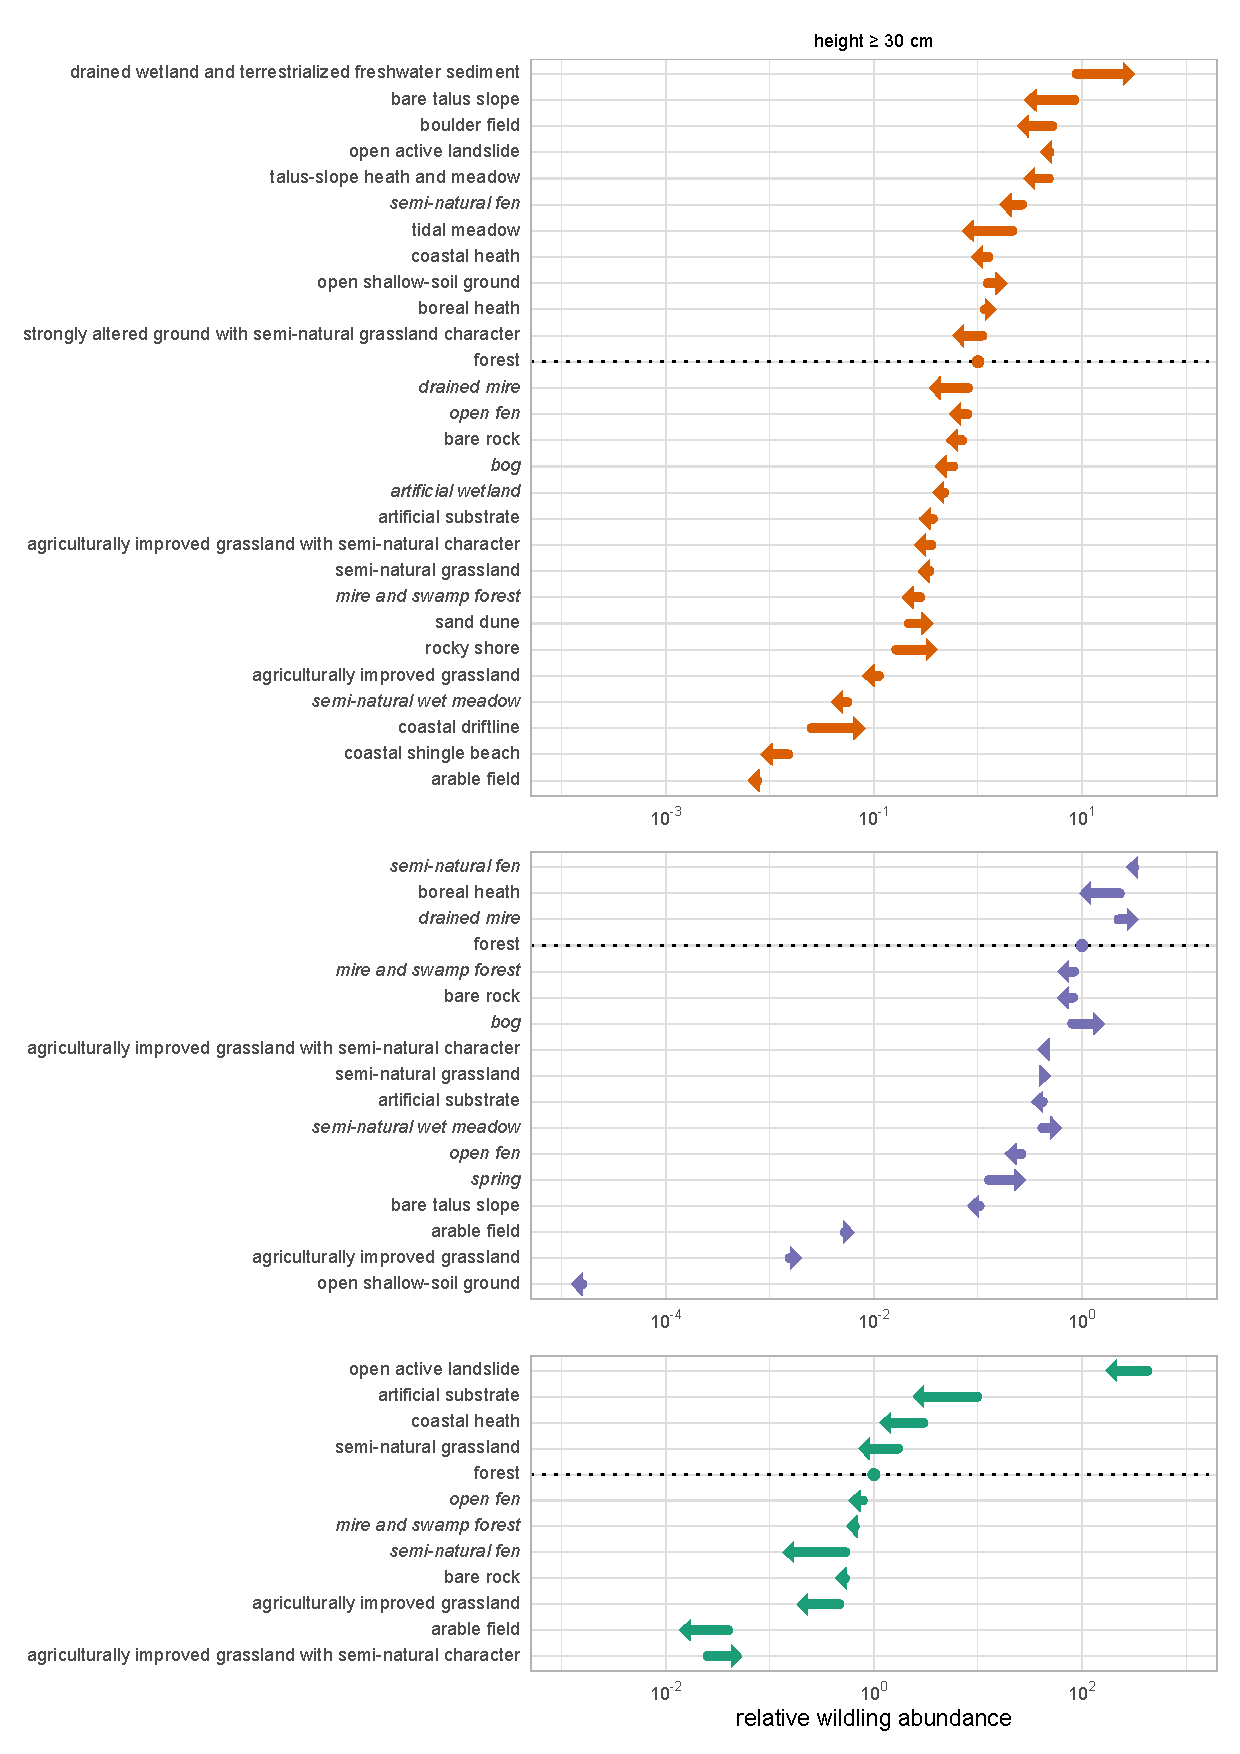
\includegraphics{figures/susceptibility-sensitivity-offset.pdf}
\caption{\label{fig:sensitivity-offset}Shifts in estimated susceptibility when relative seed rain (from the WALD dispersal model) is included in the model as a covariate rather than an offset. Arrows point from the models with offsets to the models with covariates.}
\end{figure}

\begin{figure}
\centering
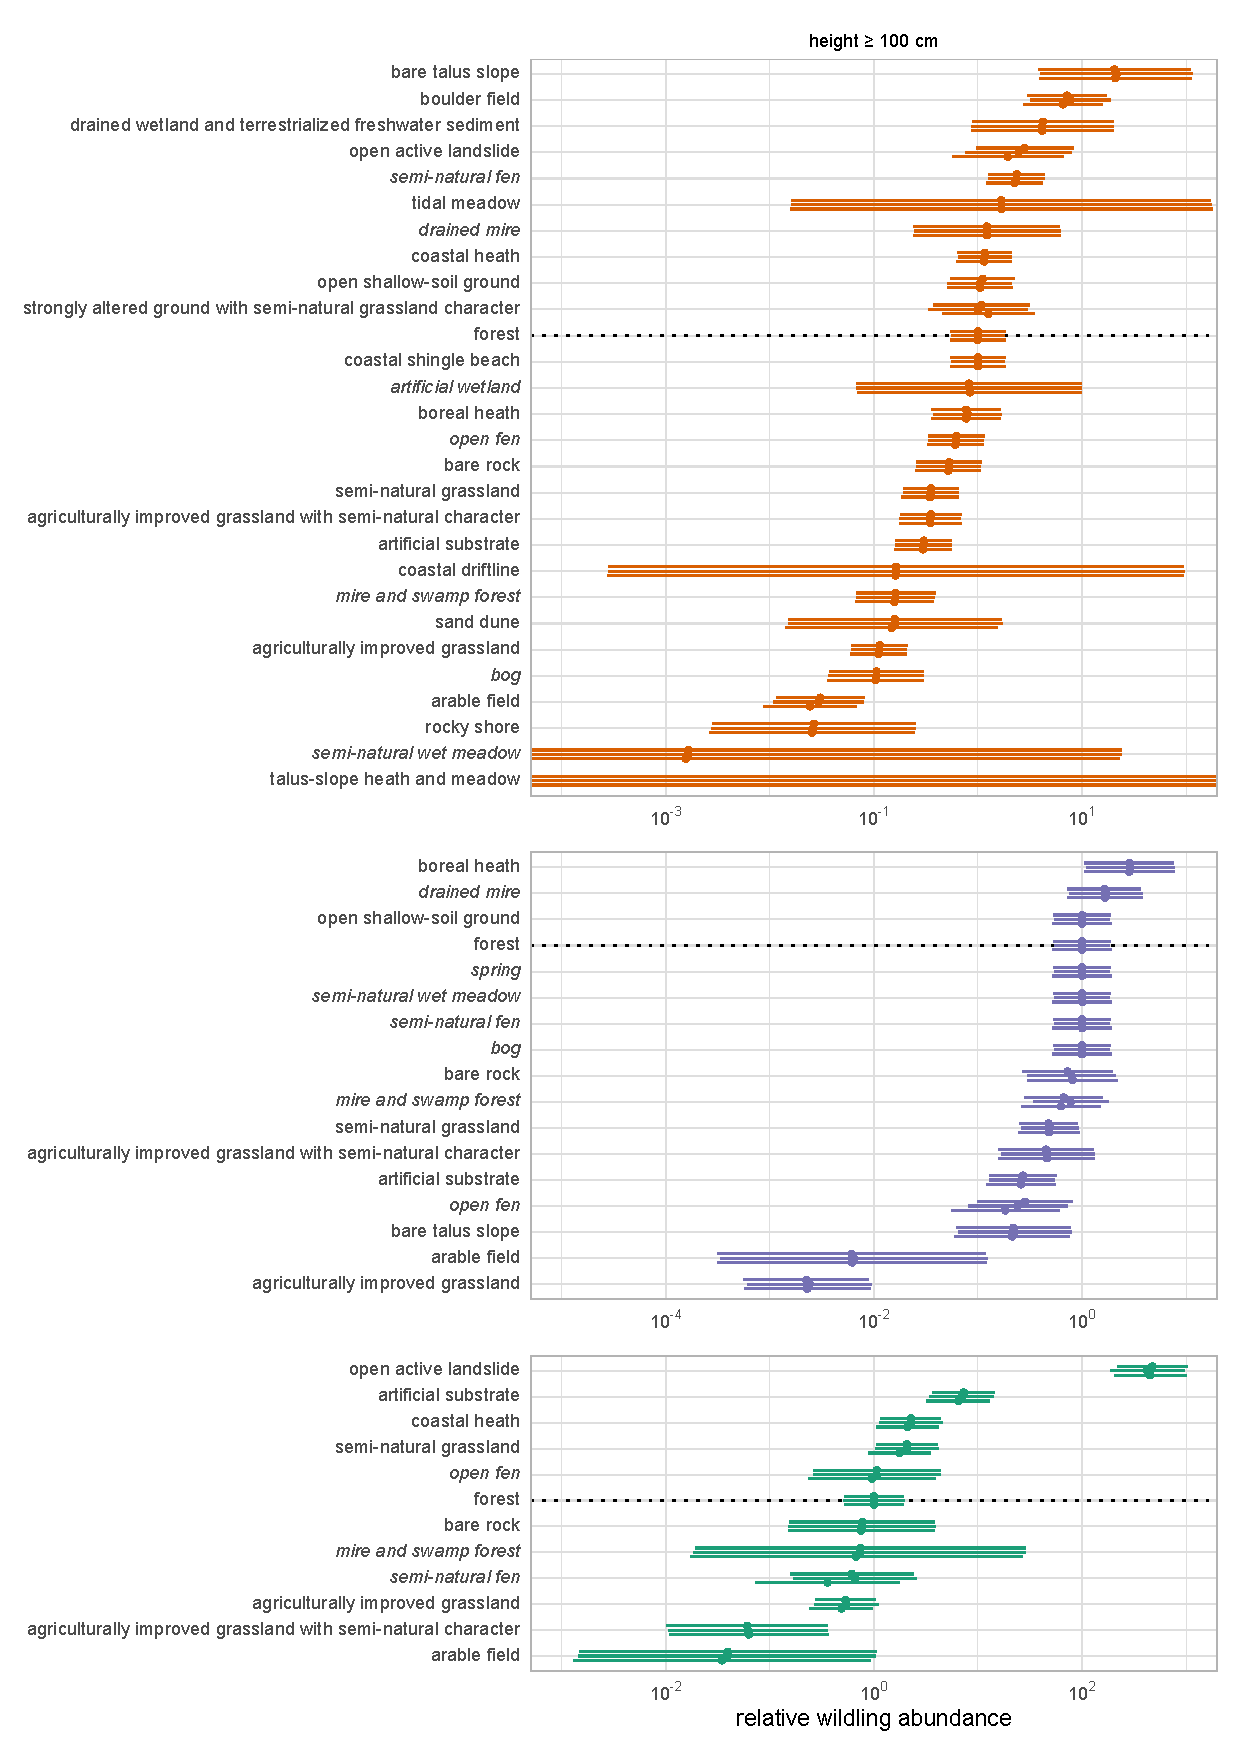
\includegraphics{figures/susceptibility-sensitivity-randomseed.pdf}
\caption{\label{fig:sensitivity-seed}Variation in estimated susceptibility to wildlings with height \(\geq\)~100~cm as a function of height assignment to unmeasured individuals. The three estimates for each ecosystem type represent three random seeds used during height assignment.}
\end{figure}

\section*{References}\label{references}
\addcontentsline{toc}{section}{References}

\phantomsection\label{refs}
\begin{CSLReferences}{1}{0}
\bibitem[\citeproctext]{ref-albertLanduseChangeSubalpine2008}
Albert, C. H., Thuiller, W., Lavorel, S., Davies, I. D., \& Garbolino, E. (2008). Land-use change and subalpine tree dynamics: Colonization of {Larix} decidua in {French} subalpine grasslands. \emph{Journal of Applied Ecology}, \emph{45}(2), 659--669. \url{https://doi.org/10.1111/j.1365-2664.2007.01416.x}

\bibitem[\citeproctext]{ref-appelgrenKartleggingAvKortdistansespredning2018}
Appelgren, L. (2018). \emph{Kartlegging av kortdistansespredning av fremmede bartrær i {Rogaland} 2018} (644). {Ecofact}.

\bibitem[\citeproctext]{ref-appelgrenKartleggingAvKortdistansespredning2017}
Appelgren, L., \& Torvik, S. E. (2017). \emph{Kartlegging av kortdistansespredning av fremmede bartrær i {Rogaland} og {Hordaland}} (607). {Ecofact}.

\bibitem[\citeproctext]{ref-arifApplyingStructuralCausal2023}
Arif, S., \& MacNeil, M. A. (2023). Applying the structural causal model framework for observational causal inference in ecology. \emph{Ecological Monographs}, \emph{93}(1), e1554. \url{https://doi.org/10.1002/ecm.1554}

\bibitem[\citeproctext]{ref-artsdatabankenFremmedartslista20182018}
Artsdatabanken. (2018). \emph{Fremmedartslista 2018}. \url{https://artsdatabanken.no/fremmedartslista2018}

\bibitem[\citeproctext]{ref-bakkestuenSteplessModelsRegional2008}
Bakkestuen, V., Erikstad, L., \& Halvorsen, R. (2008). Step-less models for regional environmental variation in {Norway}. \emph{Journal of Biogeography}, \emph{35}(10), 1906--1922. \url{https://doi.org/10.1111/j.1365-2699.2008.01941.x}

\bibitem[\citeproctext]{ref-bianchiMethodsPredictingSitka2019}
Bianchi, S., Hale, S., \& Gibbons, J. (2019). Methods for predicting {Sitka} spruce natural regeneration presence and density in the {UK}. \emph{iForest - Biogeosciences and Forestry}, \emph{12}(3), 279--288. \url{https://doi.org/10.3832/ifor2888-012}

\bibitem[\citeproctext]{ref-bindewaldSiteSpecificRisk2021}
Bindewald, A., Brundu, G., Schueler, S., Starfinger, U., Bauhus, J., \& Lapin, K. (2021). Site‐specific risk assessment enables trade‐off analysis of non‐native tree species in {European} forests. \emph{Ecology and Evolution}, \emph{11}(24), 18089--18110. \url{https://doi.org/10.1002/ece3.8407}

\bibitem[\citeproctext]{ref-blasco-morenoWhatDoesZero2019}
Blasco‐Moreno, A., Pérez‐Casany, M., Puig, P., Morante, M., \& Castells, E. (2019). What does a zero mean? Understanding false, random and structural zeros in ecology. \emph{Methods in Ecology and Evolution}, \emph{10}(7), 949--959. \url{https://doi.org/10.1111/2041-210X.13185}

\bibitem[\citeproctext]{ref-brightEvaluatingTerrestrialCarbon2020}
Bright, R. M., Allen, M., Antón‐Fernández, C., Belbo, H., Dalsgaard, L., Eisner, S., Granhus, A., Kjønaas, O. J., Søgaard, G., \& Astrup, R. (2020). Evaluating the terrestrial carbon dioxide removal potential of improved forest management and accelerated forest conversion in {Norway}. \emph{Global Change Biology}, \emph{26}(9), 5087--5105. \url{https://doi.org/10.1111/gcb.15228}

\bibitem[\citeproctext]{ref-brooksStatisticalModelingPatterns2019}
Brooks, M. E., Kristensen, K., Darrigo, M. R., Rubim, P., Uriarte, M., Bruna, E., \& Bolker, B. M. (2019). Statistical modeling of patterns in annual reproductive rates. \emph{Ecology}, \emph{100}(7), e02706. \url{https://doi.org/10.1002/ecy.2706}

\bibitem[\citeproctext]{ref-brooksGlmmTMBBalancesSpeed2017}
Brooks, M. E., Kristensen, K., van Benthem, K. J., Magnusson, A., Berg, C. W., Nielsen, A., Skaug, H. J., Maechler, M., \& Bolker, B. M. (2017). {glmmTMB} balances speed and flexibility among packages for zero-inflated generalized linear mixed modeling. \emph{The R Journal}, \emph{9}(2), 378--400. \url{https://journal.r-project.org/archive/2017/RJ-2017-066/index.html}

\bibitem[\citeproctext]{ref-brunduGlobalGuidelinesSustainable2020}
Brundu, G., Pauchard, A., Pyšek, P., Pergl, J., Bindewald, A. M., Brunori, A., Canavan, S., Campagnaro, T., Celesti-Grapow, L., de Sá Dechoum, M., Dufour-Dror, J.-M., Essl, F., Flory, S. L., Genovesi, P., Guarino, F., Guangzhe, L., Hulme, P. E., Jager, H., Kettle, C. J., \ldots{} Richardson, D. M. (2020). Global guidelines for the sustainable use of non-native trees to prevent tree invasions and mitigate their negative impacts. \emph{Neobiota}, \emph{61}, 65--116. \url{https://doi.org/10.3897/neobiota.61.58380}

\bibitem[\citeproctext]{ref-brynVeilederKartleggingAv2015}
Bryn, A., \& Halvorsen, R. (2015). \emph{Veileder for kartlegging av terrestrisk naturvariasjon etter {NiN} 2.0. Veileder versjon 2.0.0.} {Norwegian Biodiversity Information Facility}.

\bibitem[\citeproctext]{ref-bullockAllDispersalFunctions2018}
Bullock, J. M., Hooftman, D. A. P., Tamme, R., Götzenberger, L., Pärtel, M., González, L. M., \& White, S. M. (2018). All dispersal functions are wrong, but many are useful: {A} response to {Cousens} et al. \emph{Journal of Ecology}, \emph{106}(3), 907--910. \url{https://doi.org/10.1111/1365-2745.12890}

\bibitem[\citeproctext]{ref-bullockSynthesisEmpiricalPlant2017}
Bullock, J. M., Mallada González, L., Tamme, R., Götzenberger, L., White, S. M., Pärtel, M., Hooftman, D. A. P., \& Rees, M. (2017). A synthesis of empirical plant dispersal kernels. \emph{Journal of Ecology}, \emph{105}(1), 6--19. \url{https://doi.org/10.1111/1365-2745.12666}

\bibitem[\citeproctext]{ref-burnsSilvicsNorthAmerica1990}
Burns, R. M., \& Honkala, B. H. (Eds.). (1990). \emph{Silvics of {North America}. {Volume} 1, {Conifers}.} (Vol. 1). {Forest Service, USDA}.

\bibitem[\citeproctext]{ref-catfordQuantifyingLevelsBiological2012}
Catford, J. A., Vesk, P. A., Richardson, D. M., \& Pyšek, P. (2012). Quantifying levels of biological invasion: Towards the objective classification of invaded and invasible ecosystems. \emph{Global Change Biology}, \emph{18}(1), 44--62. \url{https://doi.org/10.1111/j.1365-2486.2011.02549.x}

\bibitem[\citeproctext]{ref-chaeVulnerabilityResilienceUse2021}
Chae, D. H., Snipes, S. A., Chung, K. W., Martz, C. D., \& LaVeist, T. A. (2021). Vulnerability and {Resilience}: {Use} and {Misuse} of {These Terms} in the {Public Health Discourse}. \emph{American Journal of Public Health}, \emph{111}(10), 1736--1740. \url{https://doi.org/10.2105/AJPH.2021.306413}

\bibitem[\citeproctext]{ref-chytrySeparatingHabitatInvasibility2008}
Chytrý, M., Jarošík, V., Pyšek, P., Hájek, O., Knollová, I., Tichý, L., \& Danihelka, J. (2008). Separating habitat invasibility by alien plants from the actual level of invasion. \emph{Ecology}, \emph{89}(6), 1541--1553. \url{https://doi.org/10.1890/07-0682.1}

\bibitem[\citeproctext]{ref-chytryHabitatInvasionsAlien2008}
Chytrý, M., Maskell, L. C., Pino, J., Pyšek, P., Vilà, M., Font, X., \& Smart, S. M. (2008). Habitat invasions by alien plants: A quantitative comparison among {Mediterranean}, subcontinental and oceanic regions of {Europe}. \emph{Journal of Applied Ecology}, \emph{45}(2), 448--458. \url{https://doi.org/10.1111/j.1365-2664.2007.01398.x}

\bibitem[\citeproctext]{ref-colauttiPropagulePressureNull2006}
Colautti, R. I., Grigorovich, I. A., \& MacIsaac, H. J. (2006). Propagule pressure: A null model for biological invasions. \emph{Biological Invasions}, \emph{8}(5), 1023--1037. \url{https://doi.org/10.1007/s10530-005-3735-y}

\bibitem[\citeproctext]{ref-dovciakSeedRainEnvironmental2008}
Dovčiak, M., Hrivnák, R., Ujházy, K., \& Gömöry, D. (2008). Seed rain and environmental controls on invasion of {Picea} abies into grassland. \emph{Plant Ecology}, \emph{194}(1), 135--148. \url{https://doi.org/10.1007/s11258-007-9280-2}

\bibitem[\citeproctext]{ref-esslSelectionCommercialForestry2010}
Essl, F., Moser, D., Dullinger, S., Mang, T., \& Hulme, P. E. (2010). Selection for commercial forestry determines global patterns of alien conifer invasions. \emph{Diversity and Distributions}, \emph{16}(6), 911--921. \url{https://doi.org/10.1111/j.1472-4642.2010.00705.x}

\bibitem[\citeproctext]{ref-faoGlobalForestResources2020}
FAO. (2020). \emph{Global {Forest Resources Assessment} 2020: {Key} findings}. {FAO}. \url{https://doi.org/10.4060/ca8753en}

\bibitem[\citeproctext]{ref-ForskriftOmUtsetting2012}
Forskrift om utsetting av utenlandske treslag til skogbruksformål, (2012). \url{https://lovdata.no/dokument/SF/forskrift/2012-05-25-460}

\bibitem[\citeproctext]{ref-haakenstadNORA10EIRevisedRegional2020}
Haakenstad, H., Breivik, Ø., Reistad, M., \& Aarnes, O. J. (2020). {NORA10EI}: {A} revised regional atmosphere-wave hindcast for the {North Sea}, the {Norwegian Sea} and the {Barents Sea}. \emph{International Journal of Climatology}, \emph{40}(10), 4347--4373. \url{https://doi.org/10.1002/joc.6458}

\bibitem[\citeproctext]{ref-haakenstad15yearHighResolution2017}
Haakenstad, H., \& Haugen, J. E. (2017). \emph{A 15-year high resolution meteorological dataset for risk assessment in southern {Norway}} (METreport 5/2017). {Norwegian Meteorological Institute}.

\bibitem[\citeproctext]{ref-halvorsenNaturNorgeNiN2015}
Halvorsen, R., Bryn, A., Erikstad, L., \& Lindgaard, A. (2015). \emph{Natur i {Norge} ({NiN}). Versjon 2.0.0.} {Norwegian Biodiversity Information Facility}. \url{http://www.artsdatabanken.no/naturinorge}

\bibitem[\citeproctext]{ref-halvorsenSystematicsEcodiversityEcoSyst2020}
Halvorsen, R., Skarpaas, O., Bryn, A., Bratli, H., Erikstad, L., Simensen, T., \& Lieungh, E. (2020). Towards a systematics of ecodiversity: {The EcoSyst} framework. \emph{Global Ecology and Biogeography}, \emph{29}(11), 1887--1906. \url{https://doi.org/10.1111/geb.13164}

\bibitem[\citeproctext]{ref-hartigDHARMaResidualDiagnostics2020}
Hartig, F. (2020). \emph{{DHARMa}: {Residual} diagnostics for hierarchical (multi-level / mixed) regression models} (Version 0.3.3) {[}Computer software{]}. \url{https://CRAN.R-project.org/package=DHARMa}

\bibitem[\citeproctext]{ref-higginsPineInvasionsSouthern1998}
Higgins, S. I., \& Richardson, D. M. (1998). Pine invasions in the southern hemisphere: Modelling interactions between organism, environment and disturbance. \emph{Plant Ecology}, \emph{135}(1), 79--93. \url{https://doi.org/10.1023/A:1009760512895}

\bibitem[\citeproctext]{ref-kargerClimatologiesHighResolution2017}
Karger, D. N., Conrad, O., Böhner, J., Kawohl, T., Kreft, H., Soria-Auza, R. W., Zimmermann, N. E., Linder, H. P., \& Kessler, M. (2017). Climatologies at high resolution for the earth's land surface areas. \emph{Scientific Data}, \emph{4}, 170122. \url{https://doi.org/10.1038/sdata.2017.122}

\bibitem[\citeproctext]{ref-katulMechanisticAnalyticalModels2005}
Katul, G., Porporato, A., Nathan, R., Siqueira, M., Soons, M., Poggi, D., Horn, H., \& Levin, S. (2005). Mechanistic analytical models for long-distance seed dispersal by wind. \emph{The American Naturalist}, \emph{166}(3), 368--381. \url{https://doi.org/10.1086/432589}

\bibitem[\citeproctext]{ref-kyrkjeeideKartleggingAvKortdistansespredning2017}
Kyrkjeeide, M. O., Often, A., Myklebost, H. E., Olsen, S. L., Hagelin, J., Ruano, M., Frivoll, V., \& De Stefano, M. (2017). \emph{Kartlegging av kortdistansespredning av fremmede bartrær {Nord Norge}} (1427). {NINA}.

\bibitem[\citeproctext]{ref-macekLifeDeathPicea2017}
Macek, M., Wild, J., Kopecký, M., Červenka, J., Svoboda, M., Zenáhlíková, J., Brůna, J., Mosandl, R., \& Fischer, A. (2017). Life and death of {\emph{Picea abies}} after bark-beetle outbreak: Ecological processes driving seedling recruitment. \emph{Ecological Applications}, \emph{27}(1), 156--167. \url{https://doi.org/10.1002/eap.1429}

\bibitem[\citeproctext]{ref-mcconnachieEstimatingEffectPlantations2015}
McConnachie, M. M., Wilgen, B. W. van, Richardson, D. M., Ferraro, P. J., \& Forsyth, A. T. (2015). Estimating the effect of plantations on pine invasions in protected areas: A case study from {South Africa}. \emph{Journal of Applied Ecology}, \emph{52}(1), 110--118. \url{https://doi.org/10.1111/1365-2664.12366}

\bibitem[\citeproctext]{ref-mcelreathHauntedDAGCausal2020}
McElreath, R. (2020). The {Haunted DAG} \& {The Causal Terror}. In \emph{Statisitical {Rethinking}: {A Bayesian Course} with {Examples} in {R} and {Stan}} (2nd ed.).

\bibitem[\citeproctext]{ref-miljodirektoratetUtredningAvForbud2019}
Miljødirektoratet, \& Landbruksdirektoratet. (2019). \emph{Utredning av forbud mot utsetting av utenlandske treslag til skogbruksformål} (M-1378).

\bibitem[\citeproctext]{ref-millerHowDisturbanceHistory2021}
Miller, A. D., Inamine, H., Buckling, A., Roxburgh, S. H., \& Shea, K. (2021). How disturbance history alters invasion success: Biotic legacies and regime change. \emph{Ecology Letters}, \emph{24}(4), 687--697. \url{https://doi.org/10.1111/ele.13685}

\bibitem[\citeproctext]{ref-nathanDispersalKernels2012}
Nathan, R., Klein, E., Robledo-Arnuncio, J. J., \& Revilla, E. (2012). Dispersal kernels. In J. Clobert, M. Baguette, T. G. Benton, \& J. M. Bullock (Eds.), \emph{Dispersal ecology and evolution} (pp. 187--210). {Oxford University Press Oxford}.

\bibitem[\citeproctext]{ref-nunezEcologyManagementInvasive2017}
Nuñez, M. A., Chiuffo, M. C., Torres, A., Paul, T., Dimarco, R. D., Raal, P., Policelli, N., Moyano, J., García, R. A., van Wilgen, B. W., Pauchard, A., \& Richardson, D. M. (2017). Ecology and management of invasive {Pinaceae} around the world: Progress and challenges. \emph{Biological Invasions}, \emph{19}(11), 3099--3120. \url{https://doi.org/10.1007/s10530-017-1483-4}

\bibitem[\citeproctext]{ref-nygaardNaturligSpredningAv1999}
Nygaard, P. H., Skre, O., \& Brean, R. (1999). \emph{Naturlig spredning av utenlandske treslag}. {Norsk institutt for skogforskning (NISK)}.

\bibitem[\citeproctext]{ref-nygaardSpreadIntroducedSitka2017}
Nygaard, P., \& Øyen, B.-H. (2017). Spread of the introduced {Sitka} spruce ({\emph{Picea sitchensis}}) in coastal {Norway}. \emph{Forests}, \emph{8}(1), 24. \url{https://doi.org/10.3390/f8010024}

\bibitem[\citeproctext]{ref-olsenKartleggingAvKortdistansespredning2019}
Olsen, S. L., Kyrkjeeide, M. O., Myklebost, H. E., Jackson, C., \& Gastinger, M.-M. (2019). \emph{Kartlegging av kortdistansespredning av fremmede bartrær} (1728). {NINA}.

\bibitem[\citeproctext]{ref-olsenKartleggingAvKortdistansespredning2016}
Olsen, S. L., Stabbetorp, O., Skarpaas, O., Often, A., \& Gajda, H. (2016). \emph{Kartlegging av kortdistansespredning av fremmede bartrær {Vrifuru} ({Pinus} contorta) og lutzgran ({Picea} × lutzii)} (1231). {NINA}.

\bibitem[\citeproctext]{ref-petersonEcologyManagementSitka1997}
Peterson, E. B., Peterson, N. M., Weetman, G. F., \& Martin, P. J. (1997). \emph{Ecology and management of {Sitka} spruce, emphasizing its natural range in {British Colombia}}. {UBC Press}.

\bibitem[\citeproctext]{ref-potzelsbergerGrowingNonnativeTrees2020}
Pötzelsberger, E., Spiecker, H., Neophytou, C., Mohren, F., Gazda, A., \& Hasenauer, H. (2020). Growing {Non-native Trees} in {European Forests Brings Benefits} and {Opportunities} but {Also Has Its Risks} and {Limits}. \emph{Current Forestry Reports}, \emph{6}(4), 339--353. \url{https://doi.org/10.1007/s40725-020-00129-0}

\bibitem[\citeproctext]{ref-pysekScientistsWarningInvasive2020}
Pyšek, P., Hulme, P. E., Simberloff, D., Bacher, S., Blackburn, T. M., Carlton, J. T., Dawson, W., Essl, F., Foxcroft, L. C., Genovesi, P., Jeschke, J. M., Kühn, I., Liebhold, A. M., Mandrak, N. E., Meyerson, L. A., Pauchard, A., Pergl, J., Roy, H. E., Seebens, H., \ldots{} Richardson, D. M. (2020). Scientists' warning on invasive alien species. \emph{Biological Reviews}, \emph{95}(6), 1511--1534. \url{https://doi.org/10.1111/brv.12627}

\bibitem[\citeproctext]{ref-rcoreteamLanguageEnvironmentStatistical2020}
R Core Team. (2020). \emph{R: A language and environment for statistical computing} (Version 3.6) {[}Computer software{]}. {R Foundation for Statistical Computing}. \url{https://www.r-project.org/}

\bibitem[\citeproctext]{ref-reistadHighresolutionHindcastWind2011}
Reistad, M., Breivik, Ø., Haakenstad, H., Aarnes, O. J., Furevik, B. R., \& Bidlot, J.-R. (2011). A high-resolution hindcast of wind and waves for the {North Sea}, the {Norwegian Sea}, and the {Barents Sea}. \emph{Journal of Geophysical Research: Oceans}, \emph{116}, C05019. \url{https://doi.org/10.1029/2010JC006402}

\bibitem[\citeproctext]{ref-richardsonPlantInvasionsMerging2006}
Richardson, D. M., \& Pyšek, P. (2006). Plant invasions: Merging the concepts of species invasiveness and community invasibility. \emph{Progress in Physical Geography}, \emph{30}(3), 409--431.

\bibitem[\citeproctext]{ref-richardsonConifersInvasiveAliens2004}
Richardson, D. M., \& Rejmánek, M. (2004). Conifers as invasive aliens: A global survey and predictive framework. \emph{Diversity and Distributions}, \emph{10}(5), 321--331. \url{https://doi.org/10.1111/j.1366-9516.2004.00096.x}

\bibitem[\citeproctext]{ref-rougetInferringProcessPattern2003}
Rouget, M., \& Richardson, D. M. (2003). Inferring process from pattern in plant invasions: A semimechanistic model incorporating propagule pressure and environmental factors. \emph{The American Naturalist}, \emph{162}(6), 713--724. \url{https://doi.org/10.1086/379204}

\bibitem[\citeproctext]{ref-sandvenKartleggingAvKortdistansespredning2019}
Sandven, J., Aamodt, O. W., \& Sørhuus, Ø. (2019). \emph{Kartlegging av kortdistansespredning av fremmede bartrær i {Hordaland}} (6/2019). {NORSKOG}.

\bibitem[\citeproctext]{ref-savillPlantationSilvicultureEurope1997}
Savill, P., Evans, J., Auclair, D., \& Falck, J. (1997). \emph{Plantation {Silviculture} in {Europe}}. {Oxford University Press, UK}. \url{https://books.google.com?id=ry8SgG1y6egC}

\bibitem[\citeproctext]{ref-skarpaasDispersalPatternsDispersal2007}
Skarpaas, O., \& Shea, K. (2007). Dispersal patterns, dispersal mechanisms, and invasion wave speeds for invasive thistles. \emph{The American Naturalist}, \emph{170}(3), 421--430. \url{https://doi.org/10.1086/519854}

\bibitem[\citeproctext]{ref-taylorDriversPlantInvasion2016}
Taylor, K. T., Maxwell, B. D., Pauchard, A., Nuñez, M. A., Peltzer, D. A., Terwei, A., \& Rew, L. J. (2016). Drivers of plant invasion vary globally: Evidence from pine invasions within six ecoregions. \emph{Global Ecology and Biogeography}, \emph{25}(1), 96--106. \url{https://doi.org/10.1111/geb.12391}

\bibitem[\citeproctext]{ref-teururakaunewzealandforestserviceOneBillionTrees2018}
Te Uru Rākau New Zealand Forest Service. (2018). \emph{The {One Billion Trees Programme}: Our future, our billion trees}. \url{http://www.teururakau.govt.nz/}

\bibitem[\citeproctext]{ref-textorRobustCausalInference2016}
Textor, J., van der Zander, B., Gilthorpe, M. S., Liśkiewicz, M., \& Ellison, G. T. (2016). Robust causal inference using directed acyclic graphs: The {R} package {``dagitty.''} \emph{International Journal of Epidemiology}, \emph{45}(6), 1887--1894. \url{https://doi.org/10.1093/ije/dyw341}

\bibitem[\citeproctext]{ref-tingstadTemperaturePrecipitationBiotic2015}
Tingstad, L., Olsen, S. L., Klanderud, K., Vandvik, V., \& Ohlson, M. (2015). Temperature, precipitation and biotic interactions as determinants of tree seedling recruitment across the tree line ecotone. \emph{Oecologia}, \emph{179}(2), 599--608. \url{https://doi.org/10.1007/s00442-015-3360-0}

\bibitem[\citeproctext]{ref-westreichTableFallacyPresenting2013}
Westreich, D., \& Greenland, S. (2013). The {Table} 2 {Fallacy}: Presenting and interpreting confounder and modifier coefficients. \emph{American Journal of Epidemiology}, \emph{177}(4), 292--298. \url{https://doi.org/10.1093/aje/kws412}

\bibitem[\citeproctext]{ref-zuurMixedEffectsModels2009}
Zuur, A. F., Ieno, E. N., Walker, N., Saveliev, A. A., \& Smith, G. M. (2009). \emph{Mixed effects models and extensions in ecology with {R}} (M. Gail, K. Krickeberg, J. Samet, A. Tsiatis, \& W. Wong, Eds.). {Springer New York}. \url{https://doi.org/10.1007/978-0-387-87458-6}

\end{CSLReferences}

\end{document}
